\documentclass[times, utf8, diplomski, numeric]{fer}
\usepackage{booktabs}

\usepackage{pdfpages}
\usepackage{subcaption}
\usepackage{listings}
\usepackage[toc,page]{appendix}

\graphicspath{ {images/} }

\newcommand{\eng}[1]{(engl. \textit{#1})}

\begin{document}

\thesisnumber{1385}

\title{Implementacija kontinuirane isporuke programske podrške za operacijski sustav iOS}

\author{Ivan Rep}

\maketitle

% Ispis stranice s napomenom o umetanju izvornika rada. Uklonite naredbu \izvornik ako želite izbaciti tu stranicu.
\izvornik

% Dodavanje zahvale ili prazne stranice. Ako ne želite dodati zahvalu, naredbu ostavite radi prazne stranice.
\zahvala{}

\tableofcontents

\chapter{Uvod}
Uvod rada. Nakon uvoda dolaze poglavlja u kojima se obrađuje tema.



\chapter{Kontinuirana integracija} \label{KontinuiranaIntegracija}

Kontinuirana integracija je praksa spajanja razvojnih kopija koda s glavnom kopijom nekoliko puta dnevno. Termin je prvi predložio i iskoristio Grady Booch 1991. godine tijekom opisa metode danas poznate kao Boochova metoda \eng{Booch method}\citep{wiki:BoochMethod}.

Glavni cilj metode je smanjivanje broja konflikata prilikom spajanja različitih verzija koda. Tijekom razvoja programeri preuzimaju zajedničku \eng{master} kopiju izvornog koda \eng{source code} te nad njom obavljaju promjene. Lokalnu kopiju izvornog koda nazivamo \textit{razvojnom kopijom izvornog koda}. Svaki programer ima vlastitu razvojnu kopiju izvornog koda.

Nakon implementacije željenih promjena programer vlastitu razvojnu kopiju spaja s izvornom kopijom. Ovaj postupak nazivamo integracija izvornog koda. Ako zajednička kopija izvornog koda nije bila mijenjana od kako ju je programer preuzeo, onda je promjene moguće jednostavno dodati na vrh zajedničke kopije. Međutim, ako je zajednička kopija izvornog koda izmijenjena, onda je potrebno na neki način spojiti lokalne i već spojene promjene.

Čim je duže programerova kopija izdvojena to je veća vjerojatnost izmijene izvorne kopije. Što se kopije više razlikuju to je teže obaviti njihovo spajanje. Dodatno, spajanje često nije moguće obaviti automatski. Ova se pojava naziva konflikt te se javlja prilikom spajanja kopija koje su modificirale isti dio izvornog koda. Programer u takvom slučaju prije integracije prvo mora preuzeti glavnu kopiju, ručno otkloniti konflikte koje prouzrokuju njegove promjene, te tada obaviti integraciju.

Nakon nekog vremena kopije mogu postati toliko različite da je vrijeme potrebno za njihovo spajanje duže od vremena koje je uloženo za implementaciju promjena. Ovaj se problem tada naziva \textit{pakao integracije}. Iako se ova situacija čini teško mogućom timovi mogu biti veliki, pritisak može biti visok i tempo naporan. Bez specificiranja postupka verzioniranja te automatizacije izgradnje i provjere ispravnosti projekti lako mogu završiti upravo u navedenom stanju.

Danas je kontinuirana integracija standardna praksa u razvoju programske potpore. Međutim, ona se značajno razlikuje od prakse koju je 1991. godine predložio Grady Booch. Danas se uz kontinuiranu integraciju usko vežu procesi automatizacije izgradnje i testiranja programske potpore. Ovi pojmovi su postali toliko standardan dio kontinuirane integracije da mnogi upravo njih nazivaju kontinuiranom integracijom. Drugim riječima, pojam kontinuirane integracije danas podrazumijeva barem neku razinu automatizacije procesa izgradnje i testiranje. S druge strane, učestalom spajanju radnih kopija se daje malo pozornosti.

Kontinuiranu integraciju dijelim na tri faze: izgradnju, testiranje i osiguranje kvalitete. Podjelu kontinuirane integracije na faze s podfazama je prikazana na slici \ref{fig:CIFazes}. Svaka od faza je obrađena zasebnim odlomkom u nastavku poglavlja.

\begin{figure}
\centering
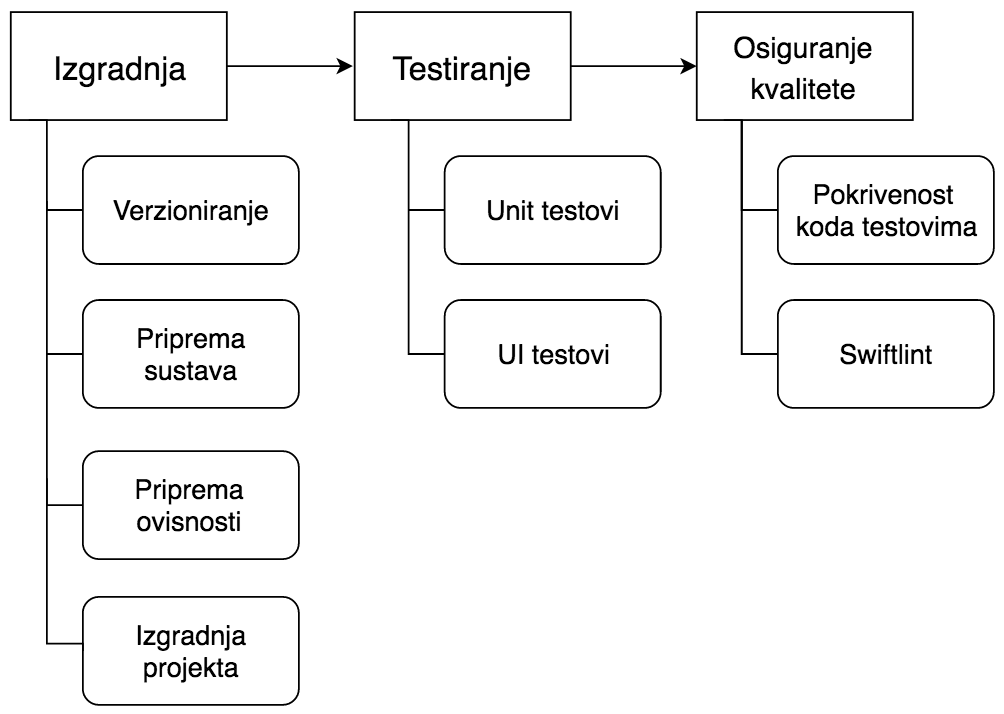
\includegraphics[scale=0.6]{CIFazes}
\caption{Faze kontinuirane integracije}
\label{fig:CIFazes}
\end{figure}

Proces verzioniranja se u praksi smatra dijelom procesa izgradnje. Zbog navedenog ću u sklopu odlomka \ref{Izgradnja} razmotriti i problem učestalosti obavljanja integracije.

Zadnji odlomak poglavlja prikazuje proces automatizacije faza korištenjem alata Xcode Server.

\section{Izgradnja} \label{Izgradnja}

Povijesno, pojam izgradnja se često koristio kao sinonim pojma kompajliranje. Kompajliranje \eng{compilation} je proces prevođenja koda iz jednog jezika u drugi uz očuvanje izvorne funkcionalnosti. Kod se prilikom prevođenja često optimizira. Najčešći razlog kompajliranja je prevođenje koda u jezik kojeg može razumjeti i time izvršiti procesor. Rezultat ovog tipa kompajliranja je izvršni program, odnosno program koji se može izvršiti. Kompajliranje je složena funkcija koja se najčešće obavlja u više prolaza. Jezici koji se kompajliraju se nazivaju kompajlirani jezici \eng{compiled languages}.

Interpretirani jezici \eng{interpreted languages} se ne prevode već interpretiraju. Oni se izvršavaju na pomoćnom programu naziva interpreter koji naredbe izvornog jezika prevodi i izvršava na računalu. Danas gotovo niti jedan jezik nije u cijelosti kompajliran ili interpretiran, već koristi kombinaciju obje metode s ciljem optimizacije performansi.

\begin{figure}
\centering
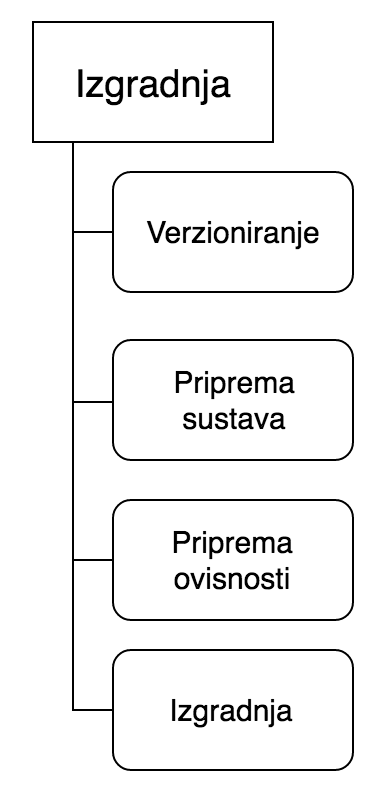
\includegraphics[scale=0.5]{BuildProcess}
\caption{Generalna podjela procesa izgradnje}
\label{fig:BuildProcess}
\end{figure}

Danas s pojmom izgradnje vežemo sve procese koji su dio pretvaranja izvornog koda u željeni artefakt. Ovisno o jeziku i alatima koje koristimo, proces izgradnje može značajno oscilirati u svojoj veličini. Generalno proces izgradnje možemo podijeliti na verzioniranje, pripremu sustava za izgradnju, dohvat i pripremu ovisnosti \eng{dependancies} te kompajliranje. Verzioniranjem odabiremo željenu verziju izvornog koda koju koristimo za izgradnju artefakta. Priprema za izgradnju dovodi računalo u stanje potrebno za obavljanje izgradnje. Izvorni kod često sadržava upute za pripremu sustava kao što su potrebni alati, ovisnosti i postavke projekta. Dohvat i priprema ovisnosti osigurava postojanje ispravnih ovisnosti korištenih u izvornom kodu. Ovisnosti dijelimo na dva tipa, službene ovisnosti koje smatramo dijelom razvojne okoline i vanjske \eng{third party} ovisnosti, najčešće razvijene od strane zajednice. Kompajliranje prevodi izvorni kod u izvršivi artefakt. Kod interpretiranih jezika ovaj je proces često zamijenjen statičkom i dinamičkom provjerom izvedivosti programa. Zbog jednostavnijeg sporazumijevanja oba procesa nazivam izgradnja projekta. Proces izgradnje je prikazan na slici \ref{fig:BuildProcess}.

Osim kreiranja željenog artefakta, izgradnja provjerava i je li zadana verzija izvornog koda izgradiva. Kod je izgradiv ako se u procesu izgradnje ne desi pogreška, odnosno ako se isti ispravno izvrši. Pogrešku može izazvati neispravnost u izvornom kodu, neispravna konfiguracija sustava, nepostojanje potrebnog alata ili neki drugi nedostatak. Izgradivost sustava je preduvjet za  testiranja i isporuku. Samim time je automatizacija izgradnje preduvjet za automatizaciju testiranja i automatizaciju isporuke.

Nastavak odlomka promatra svaki dio izgradnje zasebno. Dodatak \ref{IntegracijaDodatakA} dublje ulazi u tehničke aspekte pojedinog procesa.

\subsection{Verzioniranje}

Verzioniranje je proces dodjele jedinstvene oznake stanju izvornog koda\citep{wiki:SoftwareVersioning}. Ova oznaka omogućava jedinstvenu identifikaciju pojedinog stanja programske potpore. Verzionirano stanje izvornog koda se naziva verzija.

Uz jedinstvenu oznaku i stanje izvornog koda, proces verzioniranja pohranjuje i dodatne podatke kao što su autor, datum i lokacija kreiranja verzije. Navedeni podaci omogućavaju izgradnju stabla promjena. Ako verzije poredamo kronološki po datumu obavljanja izmjena, onda svaka pojedina verzija ne treba sadržavati cijelo stanje izvornog kod. Dovoljno je samo navesti sve promjene koje su obavljene nakon zadnjeg verzioniranja. Navedeni proces ne samo da značajno smanjuje veličinu repozitorija već olakšava i praćenje izmjena. Slika \ref{fig:VersioningTree} prikazuje primjer stabla promjena. Glavni repozitorij sadrži dvije verzije izvornog. Repozitorij u navedenom stanju preuzimaju dva programera čime kreiraju lokalne repozitorije nad kojima obavljaju izmjene. Globalno stablo promjena se kreira spajanjem stabla promjena pojedine osobe.

\begin{figure}[h!]
\centering
\begin{subfigure}{.24\textwidth}
\centering

\includegraphics[scale=0.4]{VersioningTreeA}
\caption{Glavni repozitorij}
\label{fig:VersioningTreeA}
\end{subfigure}
\begin{subfigure}{.24\textwidth}
\centering

\includegraphics[scale=0.4]{VersioningTreeB}
\caption{Repozitorij A}
\label{fig:VersioningTreeB}
\end{subfigure}
\begin{subfigure}{.24\textwidth}
\centering

\includegraphics[scale=0.4]{VersioningTreeC}
\caption{Repozitorij B}
\label{fig:VersioningTreeC}
\end{subfigure}
\begin{subfigure}{.24\textwidth}
\centering
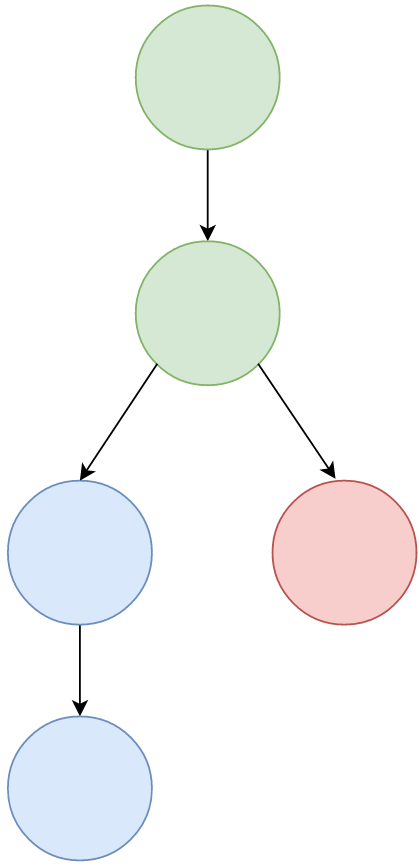
\includegraphics[scale=0.4]{VersioningTree}
\caption{Spojeni prikaz}
\label{fig:VersioningTreeD}
\end{subfigure}
\caption{Stablo promjena}
\label{fig:VersioningTree}
\end{figure}

U razvoju programske potpore se najčešće koriste dvije različite sheme verzioniranja. Unutarnje, inkrementalno verzioniranje koje se osvježava i nekoliko puta dnevno te vanjsko verzioniranje koje obilježava specifičnu verziju koda, na primjer verziju koda spremnu za objavu. Kod unutarnjeg verzioniranja sam identifikator nije bitan dokle god je on jedinstven. S druge strane, kako vanjsko verzioniranje nosi neko značenje, proces dodjele identifikatora je puno složeniji i ovisi o svrsi koje se pokušava postići. Često se za postizanje vanjskog verzioniranja dodjeljuju posebne oznake \eng{tag} unutarnjim verzijama izvornog koda.

Unutarnje verzioniranje koda se naziva kontrola verzija\citep{wiki:VersionControl}. Sustavi koji implementiraju proces kontrole verzija se nazivaju sustavi za kontrolu verzija. Kroz povijest je razvijen veliki broj sustava za kontrolu verzija te je danas timski razvoj programske potpore ne zamisliv bez korištenja jednog od ovih alata.

Danas se u praksi koriste dva alata: Apach Subversion i git. Apache Subversion, poznat i pod skraćenicom svn, je kreiran 2000. godine u sklopu projekta Apache Software Foundation zajednice. Alat je otvorenog koda, centraliziran, siguran i jednostavan za korištenje. Obično postoji jedan glavni repozitorij kojeg programeri kloniraju, uređuju te zatim lokalne promjene sinkroniziraju s glavnim repozitorijem.

Git je kreirao Linus Torvalds 2005. godine zbog nezadovoljstva tadašnjim sustavima za kontrolu verzija. Git je izdan kao alat otvorenog koda te je ubrzo okupio veliku podršku u zajednici. Za razliku od svna, git je distribuirani sustav. Repozitoriji istog projekta mogu postojati na proizvoljnom broju uređaja u proizvoljnom broju stanja. Navedeni se repozitoriji mogu klonirati, usklađivati i uređivati neovisno jedan od drugom. Zbog navedenog je pomoću gita moguće implementirati proizvoljan tijek verzioniranja. Bio to centralizirani repozitorij nalik na svnov pristup, pristup s osobama zaduženim za odobravanje promjena, distribuirani model i drugi. Najvažnije, git je jednostavan ali vrlo moćan alat. Implementacija osnovnih funkcionalnosti je jednostavna dok istovremeno postoji podrška za vrlo kompleksne pothvate.

Svn je stariji, međutim još je uvijek široko korišten sustav. Koristi ga veliki broj starijih kompanija i projekata otvorenog koda. Git je značajno dobio na popularnosti u zadnjem desetljeću. Njegova jednostavnost i fleksibilnost ga čine lakšim za upoznavanje i korištenje. Danas git preuzima tržište te se koristi u većini novih projekata. Zbog navedenog u ostatku rada koristim git. Detaljan pregled osnovnih funkcionalnosti alata git se nalazi u dodatku \ref{uvodUGit}. Sve se funkcionalnosti mogu, uz manju modifikaciju, implementirati i u svnu.

\subsection{Implementacija verzioniranja}

Ostaje otvoreno pitanje kako koristiti alat za kontrolu verzija. Koliko često kreirati novu verziju koda i koliko često promjene spajati sa zajedničkim repozitorijem. Kod korištenja gita se javljaju i pitanja kako organizirati repozitorije i sustav grananja.

Programer koji samostalno radi na projektu najčešće koristi jedan javni repozitorij s jednom granom na kojoj obavlja promjene i proizvoljno sinkronizira lokalni s glavnim repozitorijem. Međutim, ovaj pristup je vrlo teško održiv u timskom radu. Učestalo preplitanje različitih tokova razvoja na jednoj grani značajno otežava praćenje razvoja i čini teškim poništavanje neželjenih promjena.

Danas se u praksi koristi nekoliko različitih procesa verzioniranja \eng{versionining workflows}. Ovaj odlomak obrađuje centralizirani proces \eng{centralized workflow}, proces grananja funkcionalnosti \eng{feature branch workflow}, \textit{gitflow} proces \eng{gitflow workflow} i proces forkanja \eng{forking workflow}. Svaki od navedenih pristupa ima svoje prednosti i mane te se koristi u različitim tipovima projekta\citep{versioningWorkflows}.

Centralizirani proces koristi jedan glavni i više lokalnih repozitorija. Najčešće se koristi samo jedna, glavna grana. Svaki programer kreira lokalnu kopiju glavnog repozitorija na kojoj obavlja promjene. Nakon obavljanja željenih promjena iste spaja s glavnom granom centralnog repozitorija. Na pojedinom je programeru da vlastitu, lokalnu verziju repozitorija drži usklađenom s glavnim repozitorijem. Glavni repozitorij predstavlja službeno stanje projekta zbog čega treba posebnu pažnju obratiti na održavanje njegove povijesti. Izmjena povijesti glavnog repozitorija može dovesti lokalne repozitorije u nekonzistentno stanje zbog čega se ona smatra vrlo lošom praksom. Zbog navedenog, ako lokalna kopija izaziva konflikt pri spajanju, konflikt je potrebno otkloniti na lokalnoj kopiji te promjene zatim spojiti s centralnim repozitorijem. Centralizirani proces je vrlo jednostavan te je sličan načinu rada svna.

\begin{figure}[b]
\centering
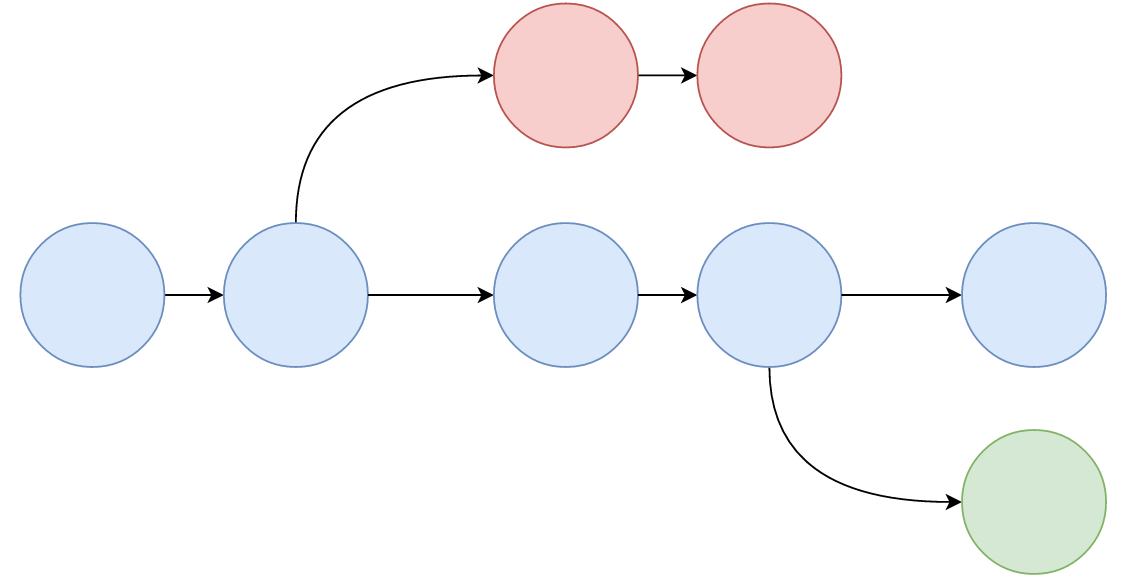
\includegraphics[scale=0.5]{FeatureBranch}
\caption{Primjer proces grananja funkcionalnosti}
\label{fig:FeatureBranch}
\end{figure}

Proces grananja funkcionalnosti nastoji otkloniti glavni nedostatak centraliziranog procesa, učestalo preplitanje različitih tokova razvoja. Proces grananja funkcionalnosti također ima jedan glavni i više lokalnih repozitorija. Razlika je u tome što se funkcionalnost implementira u grani kreiranoj specifično za nju. Programer za novu funkcionalnost kreira novu granu u lokalnom repozitoriju te u nju dodaje promjene. Po završetku implementacije funkcionalnosti programer granu spaja s glavnom granom centralnog repozitorija. Ovaj proces daje jasniji uvid u napredak projekta i implementirane funkcionalnosti. Dodatno, proces timu daje priliku revizije obavljenih promjena. Umjesto direktnog spajanja grane moguće je kreirati zahtjev za spajanjem \eng{merge request}. Zahtjev za spajanjem dodatno opisuje promjene ostvarene u sklopu grane te timu daje priliku za komunikaciju i reviziju obavljenih promjena.

Gitflow proces također koristi jedan centralni i više lokalnih repozitorija. Za razliku od prijašnja dva procesa, gitflow proces povijest repozitorija prati kroz glavnu i razvojnu granu. Razvojna grana \eng{develop branch} je vrlo slična glavnoj grani u procesu grananja funkcionalnosti. Grana za novu funkcionalnost se kreira iz razvojne grane te se po završetku implementacije u nju spaja. S druge strane, glavna grana sadrži samo produkcijske verzije izvornog koda, odnosno one verzije projekta koje su obavljene korisniku. Kad tim odluči objaviti novu verziju projekta, kreira se nova grana iz trenutnog stanja razvojne grane. Nakon završetka provjere ispravnosti grana se spaja s glavnom, i po potrebi razvojnom granom. Nova verzija glavne grane se zatim objavljuje. Verzije na glavnoj grani se označavaju sa objavljenom verzijom projekta.

Primjer korištenja gitflow procesa je prikazan na slici \ref{fig:Gitflow}. Crvenom bojom je prikazana glavna grana a plavom razvoja grana. Grane funkcionalnosti, prikazane zelenom i žutom bojom se granaju iz razvojne grane te u nju spajaju. Bijelom bojom je označena grana pripreme za objavu nove verzije projekta. Nakon obavljanja pripreme za objavu grana se spaja s glavnom granom tima kreirajući novu produkcijsku verziju, te s razvojnom granom kako bi promjene nastale kod pripreme za objavu bile dodane projektu.

\begin{figure}
\centering
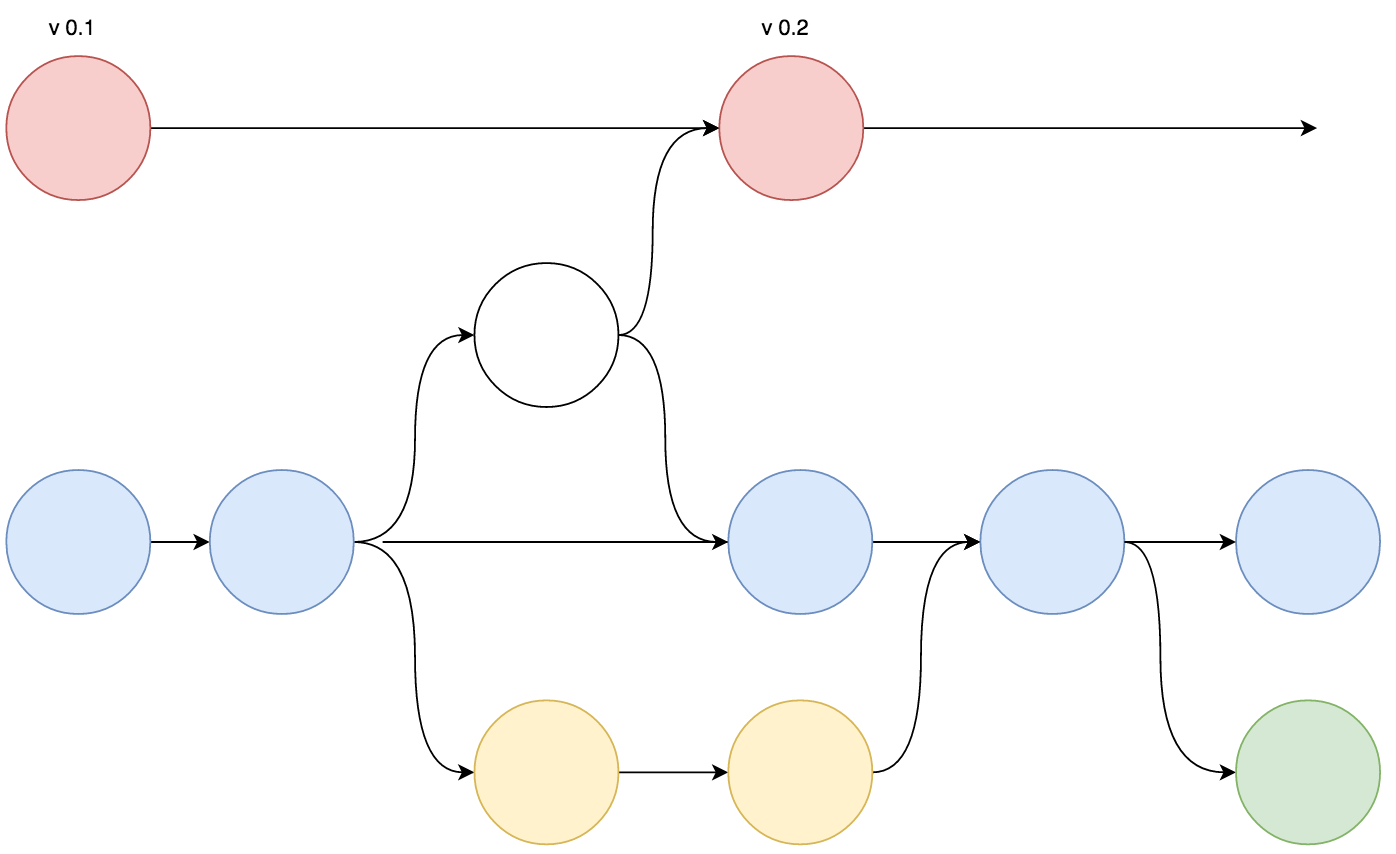
\includegraphics[scale=0.5]{Gitflow}
\caption{Primjer gitflow procesa}
\label{fig:Gitflow}
\end{figure}

Navedeni pristup olakšava upravljanje objavom projekta. Buduće da je krucijalno objaviti ispravan produkt sam proces objave treba biti kontroliran i a produkt temeljito testiran. Izdvajajući proces objave na glavnu granu omogućava istovremeno testiranje produkcijske verzije i nastavak rada na novim funkcionalnostima.

Za razliku od ostalih procesa promatranih u ovom poglavlju, forking proces nema centralni repozitorij već svaki sudionik ima vlastiti javni i privatni repozitorij. Programer vlastiti javni repozitorij kreira kopiranjem nekog drugog javnog repozitorija. Zatim iz vlastitog javnog repozitorija kreira vlastiti privatni repozitorij. Promjene obavlja na privatnom repozitoriju te ih proizvoljno spaja s javnim repozitorijem. Navedene promjene zatim može iskoristiti netko drugi kloniranjem repozitorija ili spajanjem promjena s postojećim repozitorijem. Dodatno, programer može predložiti dodavanje promjena nekom drugom repozitoriju. Navedeni se proces naziva zahtjev za povlačenjem \eng{pull request}.

Forking proces se najčešće primjenjuje za projekte otvorenog koda. On omogućuje svakom članu zajednice kloniranje, modifikaciju i objavu promjena obavljenih na projektu. Dodatno, zahtjev za spajanje daje vrlo dobar uvid u obavljene promjene bez modifikacije izvornog repozitorija.

Osnova kontinuirane integracije je kontinuirano, odnosno učestalo spajanje radnih kopija s glavnom kopijom. Kad bi se vodili samo ovim principom centralizirani repozitorij bi najbolje zadovoljavao postavljene zahtjeve. Međutim, centralizirani repozitorij se u praksi ne koristi za ništa osim najjednostavnijih projekata.

Iako drugi procesi rjeđe obavljaju integraciju radnih kopija, prednosti koje pružaju nadilaze navedeni nedostatak. Na primjer, gitflow proces integraciju radne kopije s glavnom kopijom obavlja po završetku implementacije funkcionalnosti. Što je veća funkcionalnost koja se implementira, to će duže radna kopija ostati izdvojena. Zbog navedenog je potrebno posao razdijeliti na male dijelove. Navedeno se ne odražava pozitivno samo na proces kontinuirane integracije, već olakšava i praćenje projekta te je sastavni dio agilnog pristupa razvoja programske potpore. Prednosti koje napredniji pristupi verzioniranju pruža, kao što su lakše praćenje razvoja, zahtjevi za spajanjem i lakša objava projekta u produkciju nadilaze nešto duže vrijeme izdvojenosti radnih kopija.

U praktičnom dijelu rada koristim gitflow proces. Ovaj proces najbolje odgovara zahtjevima i tipu projekta. Dodatno, gitflow proces omogućava jednostavniju implementaciju kontinuirane dostave i isporuke. Uz glavnu i radnu granu, repozitoriju ću po potrebi dodavati dodatne grane. Na primjer, isporuku verzija programske potpore za testiranje ću izdvojiti u zasebnu granu. Navedeni proces omogućava lako praćenje testnih verzija te olakšava implementaciju procesa isporuke testne verzije.

Proces kontinuirane integracije će se obavljati na svim granama. Dodatno, spajanje bilo koje dvije grane neće biti moguće ako rezultat spajanja ne prolazi sve kriterije kontinuirane integracije.

\subsection{Priprema sustava}

Priprema sustava za izgradnju se sastoji od dohvata i konfiguracije potrebnih alata te pripreme projekta za izgradnju.

Dohvat i konfiguracija alata uvelike ovisi o alatima koji se koriste u procesu izgradnje. Cilj je instalaciju i konfiguraciju što većeg broja alata automatizirati kako bi olakšali proces implementacije kontinuirane integracije. Dodatno, automatizacija procesa instalacije i konfiguracije nam omogućava instalaciju alata samo ako je to potrebno.

MacOS je vrlo siguran, i time zatvoren, operacijski sustav. Gotovo svi alati zahtijevaju korisničko dopuštenje te šifru računa koji obavlja instalaciju. Ako se instalacija obavlja za cijeli sustav ili više računa potrebno je instalaciju autorizirati računom s administracijskim privilegijama. Postoji nekoliko načina za automatski upis lozinke, ali navedeni procesi narušavaju sigurnost operacijskog sustava te ne rade za alate s grafičkim sučeljem. Zbog navedenog nije moguće u potpunosti automatizirati proces izgradnje.

Popis alata korištenih u izgradnji se nalazi u dodatku \ref{AlatiBuild}. Priprema alata čiju instalaciju nije moguće automatizirati se nalazi u dodatku \ref{PripremaAlata} dok je priprema ostalih alata specificirana u ostatku \ref{XcodeServer} dodatka.

Xcode projekt, projekt pomoću kojeg implementiram iOS aplikaciju, omogućava specifikaciju postavka izgradnje korištenjem vizualnog sučelja. Postavke izgradnje Xcode sprema u teško čitljivu formatiranu datoteku. S ciljem lakše specifikacije i praćenja postavka izgradnje se mogu iskoristiti konfiguracijske datoteke. Prilikom izgradnje postavke definirane u datotekama nadjačavaju postavke specificirane u projektu.

Za korištenje konfiguracijskih datoteka je dovoljno iste dodati projektu i repozitoriju izvornog koda. Ova je funkcionalnost posebno korisna kad je potrebno izdati više različitih verzija projekta. Na primjer, verziju za korisnika i verziju za testiranje.

\subsection{Upravljanje ovisnostima}

Prije izgradnje projekta je potrebno dohvatiti sve ovisnosti i alate koje projekt zahtjeva. Alat xcodebuild, kojeg koristimo za izgradnju programske potpore za iOS operacijske sustave, sadrži sve službene biblioteke i alate potrebne za izgradnju. Međutim, ako projekt koristi vanjske biblioteke iste je potrebno dohvatiti i pripremiti za korištenje. Za dohvaćanje vanjskih biblioteka se u iOS razvoju koriste dva alata: \textit{CocoaPods} i \textit{Carthage}.

CocoaPods je vrlo jednostavan centralizirani sustav za upravljanje ovisnostima. Za dohvaćanje ovisnosti je potrebno samo specificirati iste u datoteci imena \textit{Cartfile}. Alat samostalno kreira i konfigurira novo radno okruženje u koje dodaje osnovni projekt i sve ovisnosti. Jedino što programer mora napraviti je razvoj obavljati u radnom okruženju a ne u osnovnom projektu.

Najveći problem alata je učestala modifikacija radnog okruženja i njegovih konfiguracija. Drugim riječima, alat mijena postavke izgranje što može uzrokovati neželjeno ponašanje. Dodatno, budući da je alat centraliziran, sve korištene biblioteke moraju biti registrirane u CocoaPods sustavu. Navedeno otežava korištenje privatnih biblioteka i biblioteka u razvoju.

Carthage je decentralizirani alat za upravljanje ovisnostima. Sustav omogućava jednostavno dohvaćanje i izgradnju biblioteke. Za razliku od CocoaPods alata, Carthage ne modificira radno okruženje. Navedeno znači da je ovisnost potrebno samostalno uključiti u projekt ali u istom trenutku otklanja neželjene posljedice koje nosi CocoaPods.

Oba sustava se široko koriste te izbor uvelike ovisi o osobnom ukusu. Zbog navedenog u radu koristim oba alata.

\subsection{Izgradnja}

Izgradnja iOS aplikacija se obavlja korištenjem alat \textit{xcodebuild}\citep{xcodebuild}. Alat je razvio Apple za izgradnju programske potpore za macOS operacijski sustav. Alat je vrlo moćan te pruža veliki broj funkcionalnosti i mogućih konfiguracija. Alat je proširen te danas podržava izgradnju aplikacija za iOS, tvOS i watchOS operacijske sustave. Alat izgradnju obavlja na temelju Xcode projekta. Prije definiranje procesa izgradnje se je potrebno upoznati sa strukturom Xcode projekta.

Xcode je službeni Appleov alat za razvoj programske potpore za iOS i macOS operacijske sustave. Na tržištu postoji nekoliko alternativa ali je Xcode daleko najkorišteniji. Svi alati koriste alat xocdebuild za izgradnju te zbog toga imaju vrlo sličnu strukturu projekta. Ovaj tip projekta se naziva Xcode projekt.

Xcode projekt sadrži jedan ili više ciljeva \eng{target} i jednu ili više shema \eng{scheme}. Cilj definira postavke koji se koriste kod izvršavanja operacije za navedeni cilj.  Jedan projekt može sadržavati više ciljeva. Pomoću ciljeva je moguće isti kod distribuirati za različite verzije operacijskog sustava, različite operacijske sustave i testirati projekt. Shema definira koji se cilj koristi za koju operaciju. Projekt može implementirati više shema kako bi objedinio operacije za pojedinu distribuciju. Odnos cilja i sheme je prikazan na slici \ref{fig:TargetScheme}. Projekt sadrži tri cilja i dvije sheme. Sheme različito definiraju koji se cilj koristi za koju operaciju.

\begin{figure}
\centering
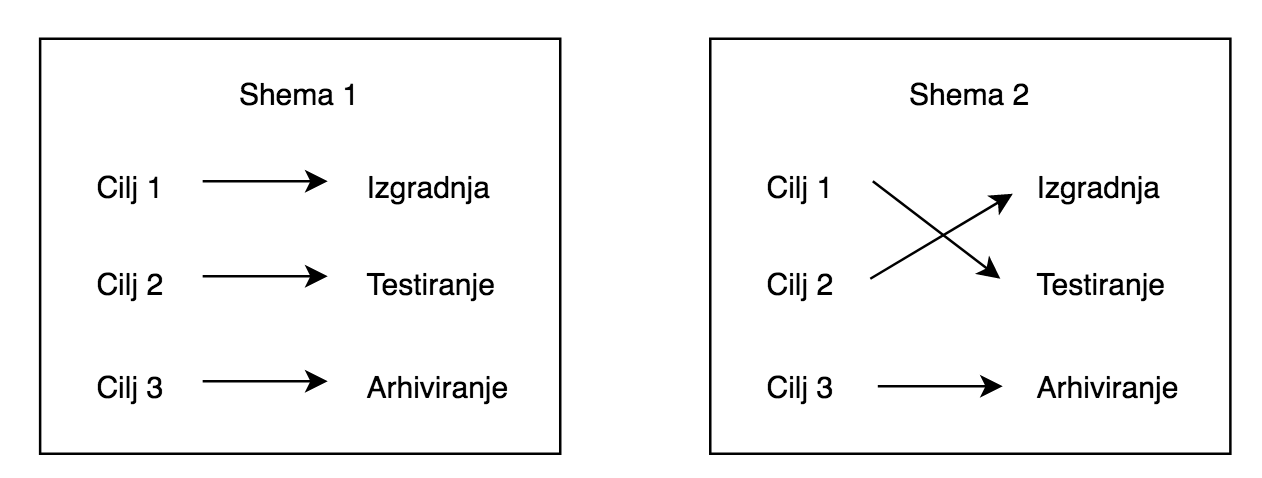
\includegraphics[scale=0.5]{TargetScheme}
\caption{Xcode projekt s tri cilja i dvije sheme}
\label{fig:TargetScheme}
\end{figure}

Xcode projekte je moguće grupirati u Xcode radno okruženje \eng{workspace}. Radno okruženje olakšava segmentiranje velikog projekta i olakšava upravljanje ovisnostima.

Pri razvoju programske potpore, operacije pokrećemo korištenjem alata Xcode. Međutim, kod automatizacije procesa naredbe možemo pozivati samo korištenjem \verb|bash| ljuske. Zbog navedenog moramo koristiti alat xcodebuild. Pokretanje alata je vrlo jednostavno. Cijeli postupak izgradnje projekta pomoću alata xcodebuild alata je prikazan u dodatku \ref{IzgradnjeDodatak}.

Ispis xcodebuild alata je vrlo detaljan. Ispis prikazuje sve izvršene naredbe te dojavljuje veliki broj međurezultata. Ovakav oblik ispisa je vrlo informativan ali je istovremeno vrlo teško čitljiv. Xcode Server, alat za automatizaciju koji koristim u ovom radu, već implementira parsiranje ispisa u lako razumljiv prikaz. U slučaju odabiri alata koji ne obavlja parsiranje  moguće je iskoristiti jedan od alata namijenjen za parsiranje xcodebuild ispisa. Trenutno je najpopularniji \textit{xcpretty} alat\citep{xcpretty}.

Proces izgradnje ne rezultira izvršivim artefaktom već samo provjerava je li sustav izgradiv. Projekt koji je izgradiv je moguće instalirati na uređaju korištenjem xcodebuild alata uz specificiranje operacije \verb|install|.

\section{Testiranje}

Testiranje je sastavni dio razvoja programske potpore. Implementacijom kvalitetnih testova ne samo da osiguravamo ispravan rad programske potpore, već sprječavamo nazadovanje koda \eng{code regression} i značajno smanjujemo potrebu za ručnim testiranjem ispravnosti\citep{wiki:SoftwareTesting}.

Pogrešno je mišljenje da implementacija testova produljuje vrijeme razvoja. Svaku implementiranu funkcionalnosti i obavljenu izmjenu je potrebno testirati. Jedino je pitanje hoće li se navedeno testiranje automatizirati ili ne. Jednom napisan kvalitetan test može se može pokrenuti beskonačan broj puta. Ručano testiranje, s druge strane, svaki put zahtijeva vrijeme zaposlenika. Bilo to u sklopu razvoja ili s ciljem provjere ispravnosti, ručna provjera ispravnosti zahtjeva više vremena i daje lošije rezultate.

Navedenu konstataciju ne treba zamijeniti s potpunim isključenjem ručnog testiranja aplikacije. Bez obzira na kvalitetu testova pogreške se uvijek mogu dogoditi. Međutim, pisanjem kvalitetnih testova se vjerojatnost pojave pogreške značajno smanjuje.

Ovaj odlomak ne ulazi u proces pisanja testova, već samo automatizira pokretanje istih. Implementacija kvalitetnih testova je vrlo složeno područje te nadilazi okvire ovog rada.

Alat xcodebuild omogućuje implementaciju dva tipa testova: Unit i UI testove.

Unit testovi su nesretno imenovani. Oni ne predstavljaju standardne unit testove, već se koriste kao ime za testove koji imaju pristup kodu koji testiraju. Testovi direktno komuniciraju s kodom koji testiraju i kroz ovu komunikaciju provjeravaju ispravnost izvođenja. Ovaj tip testa se pokreće kao omotač oko izvorne aplikacije.

S druge strane, UI testovi nemaju pristup izvornom kodu aplikacije. Oni programsku potporu testiraju njezinim pokretanjem i simuliranjem korisničke interakcije. Programer specificira korisničke akcije i ponašanje koje očekuje od aplikacije nakon primanja navede akcije. UI testovi pokreću dvije aplikacije: aplikaciju koju testiraju i aplikaciju koja simulira korisničku interakciju.

Oba tipa testova su implementirani kao testni ciljevi Xcode projekta. Kod testnog cilja nije dio produkcijskog te se ne koristi u procesu izgradnje. Testni cilj referencira cilj koji testira. Dodatno, cilj može specificirati koji se testni ciljevi pokreću prilikom pokretanja operacije testiranja. Na ovaj način jedan cilj može specificirati više testnih ciljeva te pokretanjem operacije testiranja pokrenuti sve navedene testne ciljeve. Navedeni proces olakšava pokretanje testova korištenjem xcodebuild alata.

U sklopu razvoja testiranje pokrećemo korištenjem Xcode alata. Alat obavlja sve potrebne operacije i dojavljuje rezultate procesa. Ručno pokretanje testiranja se također obavlja korištenjem alat xcodebuild.

Proces testiranja se pokreće na iOS Simulatoru, aplikaciji koja simulira iOS operacijski sustav na macOS operacijskom sustavu. Zbog navedenog je potrebno preuzeti barem jedan iOS simulator željene verzije.

Primjer naredbe koja pokreće testni proces se nalazi u dodatku \ref{TestiranjeXcodeBuild}. Ispis naredbe je sličan ispisu izgradnje te je preporučeno koristiti jedan od parsera ispisa.


\section{Osiguranje kvalitete}

Osiguranje kvalitete služi za provjeru dodatnih restrikcija koje samostalno namećemo na izvorni kod. Navedene restrikcije nastoje poboljšati kvalitetu koda, konačnog produkta i procesa razvoja. Osiguranje kvalitete može sadržavati jednostavna pravila, kao što su zahtijevanje postojanja komentara za svako spajanje, ili vrlo složena pravila koje provjeravaju specijalizirani alati.

Dodatno, moguće je obavljati različite provjere za različite tipove konačnog produkta. Na primjer, produkt koji izdajemo u produkciju mora biti vrlo kvalitetan i strogo istestiran. S druge strane, kod isporuke produkta za testiranje želimo samo isporučiti trenutno stanje programske potpore ma kakva ona bila. Zbog navedenog će ova dva primjera postavljati značajno različite kriterije osiguranja kvalitete.

Navedenu je fleksibilnost moguće ostvariti na nekoliko načina. Jedan od jednostavnijih načija je unaprijed automatizirati procese osiguranja kvalitete za sve željene slučajeve te ih pozivati na temelju neke predodređene oznake, na primjer imena grane na kojoj se obavlja integracija.

U sklopu osiguranja kvalitete implementiram dvije provjere: pokrivenost koda testovima i provjeru koda korištenjem alata Swiftlint.

Pokrivenost koda testovima \eng{code coverage} je mjera koja govorili u kolikom je postotku izvorni kod pokriven testovima. Svaki redak koda koji je barem jednom izvršen u procesu testiranja je pokriven testovima. Što je navedena mjera veća to je više koda testirano. Zbog toga možemo reći da veća pokrivenost koda testovima, u generalnom slučaju, vodi k boljoj kvaliteti konačnog produkta.

Međutim, navedena se mjera može vrlo lako zloupotrijebiti. Na primjer, moguće je napisati vrlo jednostavan test koji samo pokreće aplikaciju i time poziva značajan postotak koda. Zbog navedenog se u praksi često koriste modificirane verzije mjerenja pokrivenosti koda testovima koje procesu dodaju dodatna pravila te time nastoje utvrditi stvarnu kvalitetu testiranja\citep{wiki:CodeCoverage}.

Alat xcodebuild implementira mjerenje pokrivenosti koda testovima. Dovoljno je naredbi za pokretanje testova dodati argument \verb|-showBuildSettings|. Ispis naredbe se pohranjuje kao skup datoteka koje služe za prikazivanje pokrivenosti koda testovima u alatu Xcode. Uz sam postotak pokrivenosti koda testovima, Xcode prikazuje i pokrivenost pojedinog dokumenta te broj poziva svake pojedine linije koda. Navedene datoteke nisu namijenjene za ljudsko čitanje. Primjer naredbe se nalazi u dodatku \ref{OsiguranjeKvaliteteImplementacija}.

Swiftlint je alat za statičku analizu koda napisanog u programskom jeziku Swift. Alat definira veliki broj pravila kojima nastoji osigurati praćenje stila i konvencija jezika pri pisanju koda u Swiftu\citep{SwiftLint}. Većina pravila se odnosi na izgled i format koda, ali postoje i pravila koja nastoje izbjeći pojavu grešaka. Ne poštivanje pravila izaziva dojavu upozorenja \eng{warning} ili greške \eng{error} jednake onima procesa izgradnje. Pravila je moguće modificirati, u potpunosti isključiti ili dodati nova.

Swiftlint je vrlo koristan alat. Pridržavanje strogog formata pisanja koda olakšava timski rad, poboljšava čitljivost koda i izbjegava pojavu lako izbjegnutih grešaka.

Alat se pokreće pozivanjem naredbe \verb|swiftlint| u početnom direktoriju projekta. Dodatno, moguće je Xcode projektu dodati novu \verb|Run Script| fazu koja će alat pozivati prilikom svake izgradnje te će upozorenja i greške alata Swiftlint dojaviti zajedno s ostalim upozorenjima i greškama. Navedenim postupkom izbjegavamo ručnu provjeru ispisa alata. Primjer korištenja alata je dostupan u dodatku \ref{OsiguranjeKvaliteteImplementacija}.


\section{Implementacija kontinuirane integracije} \label{XcodeServerCI}

Za ostvarenjen kontinuirane integracije je potrebno automatizirati procese navedene u ovom poglavlju. Automatizaciju procesa možemo ostvariti ručno. Potrebno bi bilo implementirati proces koji osluškuje javni git repozitorij te prilikom detekcije promjene pokreće proces integracije.

Proces integracije bi preuzeo novu verziju izvornog koda, pomoću alata CocoaPods i Carthage dohvatio ovisnosti te pomoću alata xcodebuild obavio izgradnju, testiranje i provjeru pokrivenosti koda testovima. Rezultat integracije je moguće formatirati korištenjem alata xcpretty te poslati zainteresiranim osobama korištenjem email poruke ili nekog drugog oblika komunikacije.

Međutim, na tržištu već postoji veliki broj alata koji već implementiraju navedene funkcionalnosti. Dodatno, navedeni alati pružaju i brojne funkcionalnosti kao što su formatirani prikaz rezultata, udaljeno kreiranje i konfiguriranje procesa te testiranje na stvarnim uređajima. Korištenjem ovih alata olakšavamo implementaciju kontinuirane integracije.

Za implementaciju kontinuirane integracije, dostave i isporuke koristim alat Xcode Server. Na tržištu postoji vrlo velik broj sličnih alata. Dodatak \ref{UsporedbaCIAlata_DodatakC} objašnjava zašto sam od svih alata odabrao upravo Xcode Server.

Xcode Server je izgrađen specifično za implementaciju kontinuirane integracije za Xcode projekte. Zbog navedenog je proces implementacije značajno jednostavniji u usporedbi s većinom sličnih alata.

Xcode Server je kombinacija dva alata, Xcodea i macOS Servera. Xcode je alat za razvoj programske podrške za iOS, macOS, tvOS i watchOS operacijske sustave. Alat Xcode već koristim u razvoj programske potpore. MacOS Server je alat za automatizaciju procesa na macOS operacijskom sustavu. Prvenstveno je izgrađen za lakšu automatizaciju procesa, ulančavanje poziva skripta i upravljanje udaljenim pristupom računalu. Danas brojni alati koriste macOS Server za lakše ostvarenje automatizacije. Među njima je i Xcode.

Pomoću alata Xcode kreiramo, konfiguriramo i pratimo automatizirane procese. Procesi se pohranjuju i izvršavaju na macOS Serveru. MacOS Server na kojem se pokreću procesi može biti na lokalnom ili udaljenom računalu.

Oba alata razvija Apple zbog čega su aplikacije usklađene te su nove funkcionalnosti dostupne na dan njihovog izdavanja. Dodatno, inzistiranje na jednostavnosti korištenja, bogatstvo funkcionalnosti i laka proširivost čine ovaj alat jednim od najboljih za ostvarenje kontinuirane integracije, dostave i isporuke za razvoj iOS aplikacija.

Glavni manjak Xcode Servera je ograničenost na isključivo Xcode projekte. Kako razvoj mobilnih aplikacija gotovo uvijek uključuje iOS i Android operacijske sustave, timovi se češće odluče na implementaciju zajedničkog rješenja. Dodatno, kako je svijet mobilnih aplikacija vrlo mlad, većina se timova još uvijek drži općih rješenja kao što su Jenkins ili CircleCI.

Za početak implementacije kontinuirane integracije je potrebno preuzeti alate macOS Server i Xcode. Alate je moguće preuzeti korištenjem aplikacije App Store. Cijena macOS Servera je \$25 ali je besplatan za osobe s Apple Developer računom. Navedeni račun je potreban i za izgradnju iOS aplikacija zbog čega ga već ima većina iOS programera.

Nakon instalacije je potrebno povezati alate. Povezivanje se ostvaruje odabirom opcije \verb|Xcode| u macOS Server alatu. Odabir opcije otvara novi prozor u kom je potrebno locirati i odabrati željenu verziju Xcode alata. Ovime je kreiran alat Xcode Server.

Moguće je odabrati račun operacijskog sustava na kojem će se izvršavati integracije. Zbog sigurnosti je preporučeno Xcode Server pokrenuti na zasebnom račun koji nema administrativna prava. Budući da se Xcode Serveru može pristupiti iz vanjske mreže, važno je ograničiti prava koja alat posjeduje. Izdvajanjem procesa na zasebni račun osiguravamo da alat ima samo ona prava koja su mu potrebna. Moguće je kreirati račun proizvoljnog imena, ali je standardno koristiti ime \textit{xcodeserver}. Računu na kojem se obavlja integracija je potrebno dati potrebna prava te osigurati postojanje potrebnih alata.

Budući da želimo automatizirati što veću količinu posla, poželjno je što više potrebnih alate instalirati u sklopu integracije, a ne zahtijevati njihovo prethodno postojanje na računalu. Međutim, što više funkcionalnosti nastojimo automatizirati to se implementacija integracije više komplicira. Dodatno, brojni alati za instalaciju zahtijevaju posebno dopuštenje i interakciju korisnika. Instalaciju takvih alata nije moguće automatizirati bez značajnog narušavanja sigurnosti operacijskog sustava.

U procesu integracije koristimo tri alata za olakšavanje dohvaćanja i konfiguracije drugih alata: ruby, gem i Homebrew. Alati ruby i gem su dostupni na svim instalacijama macOS operacijskog sustava. Međutim, ako su lokacije njihove instalacije promijenjena, onda je potrebno istu dodati u \verb|PATH| varijablu računa operacijskog sustava ili izmijeniti skripte kako bi iste pokazivale na ispravnu lokaciju. Alat Homebrew je potrebno ručno dohvatiti i konfigurirati. Proces je prikazan u dodatku \ref{PripremaAlata}.

Za olakšavanje implementacije kontinuirane integracije koristim alate CocoaPods, Carthage i Swiftlint. Instalacija i konfiguracija navedenih alata je prikazana u dodatku \ref{XcodeServer}.

Automatizaciju izgradnje, testiranja i osiguranja kvalitete implementiram korištenjem alata \verb|bot| koji je dio Xcode alata. Bot se kreira u alatu Xcode odabirom opcije \verb|Product -> Create bot...|. Za kreiranje je potrebno specificirati repozitorij izvornog koda te odabirati opcije integacije. Sve potrebne funkcionalnosti su već implementirane te je potrebno samo ukljućiti njihovo korištenje. Proces kreiranja bota je prikazan u dodatku \ref{KontinuiranaIntegracija_DodatakB}.

Budući da dohvat ovisnosti implementiram korištenjem alata CocoaPods i Carthage, instalaciju, konfiguraciji i pokretanje alata je potrebno samostalno automatizirati. Za automatizaciju naredba možemo iskoristiti funkcionalnost bot alata, akciju koja se obavlja prije izgradnje \eng{pre-build action}. Ove se akcije pozivaju u sklopi integracije nakon dohvaćanja izvornog koda a prije obavljanja izgradnje.

Sve naredbe koje se pozivaju u sklopu akcije je korisno izdvojiti u zasebnu skriptu. Drugim riječima, akcija jednostavno poziva skriptu koja zatim definira naredbe koje se izvršavaju. Navedeni pristup olakšava izmjenu i nadopunu naredba te ne zahtijeva izmjenu procesa integracije.





\chapter{Kontinuirana dostava}

Kontinuirana dostava je praksa koja automatizacijom procesa isporuke programske podrške nastoji omogućiti čestu i pouzdanu isporuku ispravnog produkta u produkciju. Automatizacija procesa isporuke značajno smanjuje količinu vremena koje tim mora uložiti na proces i time potiče češće izdavanje. Dodatno, implementacija jednostavnog i automatiziranog procesa isporuke smanjuje mogućnost pojave ljudske pogreške. Proces u isto vrijeme nastoji smanjiti trošak, rizik i vrijeme uloženo u razvoj te poboljšati ispravnost produkta\citep{wiki:ContinuousDelivery}.

Programsku potporu je prije isporuke potrebno izgraditi, testirati, provjeriti ispravnost te kreirati artefakt za distribuciju. Iako različiti razvojni procesi različito nazivaju artefakt za distribuciju, zbog jednostavnosti ga nazivam arhiva. Arhiviranje je proces kreiranje arhive programske potpore. Arhiva omogućava instalaciju programske potpore na operacijskom sustavu za kojeg je programska potpora namijenjena.

Jednako tako je prije automatizacije isporuke produkta potrebno automatizirati izgradnju, testiranje, provjeru ispravnosti i arhiviranje programske potpore. Proces automatizacije izgradnje, testiranja i provjere ispravnosti se naziva kontinuirana integracija te je definiran u poglavlju \ref{KontinuiranaIntegracija}. Kontinuirana dostava obuhvaća proces kontinuirane integracije te proces automatizacije isporuke.

Međutim, u praksi se pojam kontinuirana dostava češće koristi za proces automatizacije isporuke koji zahtijeva prethodnu implementaciju procesa kontinuirane integracije. Navedeni se pristup koristi u ovom radu. Proces izgradnje, testiranja i provjere ispravnosti implementiram u sklopu kontinuirane integracije na koju dodajem automatizaciju isporuke i time ostvarujem kontinuiranu dostavu.

Važno je napomenuti da kontinuirana dostava ne isporučuje produkt automatski, već samo automatizira proces isporuke. Osoba zadužena za isporuku produkta još uvijek mora pokrenuti proces isporuke za željenu verziju produkta. Automatska objava programske potpore je obrađena u sljedećem, \ref{header:KontinuiranaIsporuka} poglavlju.

Programsku potporu je moguće objaviti na više načina. Samim time postoji i više procesa isporuke. Programsku potporu je moguće isporučiti ručnom distribucijom njenih arhiva, objavom arhive na privatnom poslužitelju ili objavom arhiva na nekoj javnoj distribucijskoj platformi. Navedeni načini isporuke se značajno razliku. Samim time se i automatizacije navedenih načina isporuke značajno razlikuju.

Programsku potporu za iOS operacijski sustav isporučujemo na sljedeće načine: direktna isporuka \eng{direct distribution}, \textit{ad hoc} isporuka \eng{ad hoc distribution}, unutarnja isporuka \eng{in-house distribution} i isporuka korištenjem App Store platforme. Odabir načina uglavnom ovisi o klijentu za koji obavljamo isporuku. Na primjer, za isporuku programske potpore unutar tima možemo koristiti direktnu isporuku. Jednostavno povežemo mobilni uređaj s računalom koje obavlja isporuku i instaliramo aplikaciju. Isto naravno nije moguće te ne bi bilo praktično raditi za javne korisnike. Njima programsku potporu isporučujemo korištenjem javne App Store platforme odakle je oni mogu samostalno preuzeti. Primjer implementacije svakog od pristupa je dostupan u dodatku \ref{header:ImplementacijaIsporuke}.

Svaki od spomenutih tipova isporuke se koristi u razvoju programske potpore za iOS operacijski sustav. Zbog navedenog ću u sklopu automatizacije isporuke, odnosno kontinuirane dostave, obraditi sve navedene tipove isporuke. Iako se procesi razlikuju u implementaciji, sastoje se od istih koraka: pripreme za distribuciju, odnosno arhiviranja programske potpore i objave. Slika \ref{fig:ContinuousDelivery} prikazuje proces isporuke.

\begin{figure}
\centering
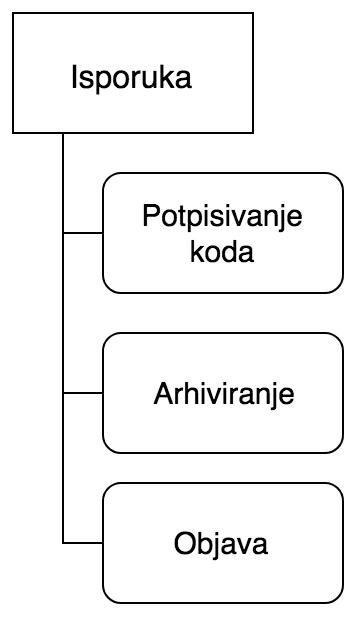
\includegraphics[scale=0.6]{ContinuousDelivery}
\caption{Proces isporuke}
\label{fig:ContinuousDelivery}
\end{figure}

\section{Potpisivanje koda}

Kako bi osigurao autentičnost i ne izmijenjenost objavljene programske potpore, Apple koristi sustav potpisivanja koda \eng{code signing}. Sustav se sastoji od dva tipa artefakta: certifikata i profila. Certifikati se sastoje od javnog i privatnog ključa te služe za potpisivanje i kriptiranje programske potpore. Profili sadrže informacije o aplikaciji i razvojnom timu te se prilikom arhiviranja dodaju programskoj potpori.

Za kreiranje arhive, a samim time i isporuku programske potpore, je potrebno posjedovati odgovarajuće certifikate i profile. U sklopu isporuke se koriste dva certifikata i jedan profil: certifikat programera koji obavlja isporuku, certifikat aplikacije koja se isporučuju te profil za aplikaciju koji odgovara tipu isporuke koji se obavlja\citep{codesigning}. Postoje četiri tipa profila od kojih svaki odgovara svom tipu isporuke: razvojni, ad hoc, unutarnji i App Store profil. Za kreiranje razvojnog, ad hoc i App Store profila je potrebno posjedovati Apple Developer račun dok je za unutarnji profil, pa samim time i unutarnju isporuku, potrebno posjedovati Apple Enterprise račun.

Certifikati i profili se kreiraju korištenjem Apple Developer platforme. Proces kreiranja i pripreme artefakta je prikazan u dodatku \ref{header:PotpisivanjeKodaDodatak}.

Ručno kreiranje i održavanje certifikati i profila se može vrlo lako zakomplicirati. Certifikati se sastoje od dva dijela, javnog i privatnog ključa. Javni ključ je moguće slobodno distribuirati. Međutim, tajni ključ je nužno održati tajnim. Drugim riječima, pristup tajnom ključu moraju imati samo osobe zadužene za njegovo korištenje. Profili su također potpisani certifikatom. Profili za razvoj su potpisani generalnim certifikatom za razvoj, dok su certifikati za isporuku potpisani certifikatima aplikacije. Zbog navedenog je uz profile potrebno distribuirati i pripadajuće privatne ključeve.

Postoji nekoliko pristupa koji olakšavaju proces potpisivanja koda. Novije verzije Xcode alata automatiziraju kreiranje i održavanje certifikati i profila koji se koriste u razvoju. Međutim, za isporuku je još uvijek potrebno samostalno kreirati potrebne artefakte. Budući da u sklopu automatiziranja kontinuirane isporuke automatiziramo i proces potpisivanja koda, moramo pronaći postupak koji automatizira kreiranje i upravljanje certifikatima i profilima.

Kako bi automatizirali potpisivanje koda moramo riješiti dva pitanja, kreiranje i dohvat profila i certifikata te kreiranje, sigurna pohrana i dohvat privatnih ključeva. Apple Developer platforma omogućava kreiranje i dohvat certifikata i profila korištenjem javnog programskog sučelja. Dodatno, nekoliko postojećih alata omogućava vrlo jednostavno korištenje programskog sučelja. Za pohranu i dohvat privatnih ključeva koristim privatni repozitorij objaven na javno dostupnoj platformi. Navedeni pristup značajno olakšava proces distribucije i kontrole pristupa privatnim ključevima.

\subsection{Automatizacija potpisivanja koda}

Kako bi automatizirali proces arhiviranja projekta, moramo automatizirati proces potpisivanja koda. U svrhu jednostavnije automatizacije razdvajamo potpisivanje koda na konfiguriranje projekta te dohvat i kreiranje artefakta potrebnih za potpisivanje.

Potpisivanje koda konfigurira projekt kako bi proces arhiviranja koristio ispravne artefakte za kreiranje arhive. Različiti tipovi isporuke zahtijevaju arhive potpisane različitim artefaktima. Zbog navedenog razloga je na temelju tipa isporuke potrebno projekt konfigurirati ispravnim artefaktima. Prije konfiguriranja projekta je artefakte potrebno dohvatiti, te ako ne postoje kreirati. Svaki od tipova isporuke zahtijeva dva certifikata, pripadajuće privatne ključeve i profil za tip isporuke koji se ostvaruje. Slika \ref{fig:CodeSigning} prikazuje podjelu potpisivanja koda.

\begin{figure}
\centering
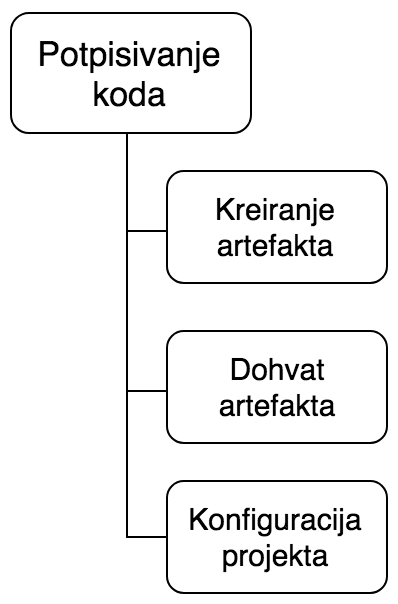
\includegraphics[scale=0.6]{CodeSigning}
\caption{Potpisivanje koda}
\label{fig:CodeSigning}
\end{figure}

Apple Developer platforma pruža javni API koji je moguće iskoristiti za kreiranje artefakta potrebnih za potpisivanje koda. Nekoliko javno dostupnih alata koriste ovaj API kako bi olakšali implementaciju kreiranja artefakta.

Kao što je navedeno u prošloj sekciji, kreirane artefakte pohranjujem u privatnom repozitoriju. Ne samo da ovaj pristup olakšava upravljanje artefaktima, već i značajno olakšava automatizaciju dohvata. Dovoljno je dohvatiti repozitorij i provjeriti postoji li potreban artefakt. Ako artefakt ne postoji isti se kreira i pohranjuje u repozitoriju.

Konfiguriranje projekta je potrebno obaviti samo nakon kreiranja novog artefakta. Zbog navedenog se proces najčešće obavlja ručno. Nakon automatskog kreiranja i dohvata artefakta, projekt se ručno konfigurira kako bi koristio ispravne artefakte. Međutim, navedeni pristup ne omogućava automatsko osvježavanje i zamjenu artefakta. Ova funkcionalnost je korisna u dva slučaja: istjecanje i ugroženost artefakta. Nakon isticanja artefakta je iste potrebno obnoviti, odnosno kreirati nove artefakte koji mijenjaju postojeće. U slučaju ugroženosti artefakta je iste potrebno povući iz uporabe te kreirati nove. Budući da su ova dva slučaja vrlo rijetka, procesa konfiguracije projekta se najčešće ne automatizira.

Automatizaciju konfiguracije projekta je najlakše ostvariti definiranjem sheme imenovanja artefakta koji se koriste u pojedinom tipu isporuke. Definiranjem sheme nazivanja i njenom primjenom proces unaprijed zna nazive potrebnih artefakta pomoću čega može konfigurirati projekt.

Automatizaciju potpisivanja koda je moguće implementirati ručno ili korištenjem nekog od postojećih alata. U sklopu ovog rada koristim alata \verb|match| koji je dio \verb|fastlane| familije. Alat implementira sve potrebne funkcionalnosti te pruža veliki broj opcija konfiguracije. Implementacija automatizacije potpisivanja koda korištenjem \verb|match| alata je prikazana u dodatku \ref{header:PotpisivanjeKodaDodatak}.

\section{Isporuka programske potpore} \label{header:RucnaIsporuka}

U sklopu razvoja programske potpore za iOS operacijski sustav se koristi četiri tipa isporuke: direktna isporuka, ad hoc isporuka, unutarnja isporuka i isporuka korištenjem App Store platforme.

Direktna isporuka aplikaciju instalira direktno na uređaj, odakle i dobiva svoje ime. Za obavljanje direktne isporuke je potrebno uređaj povezati s računalnom koje obavlja isporuku direktnom vezom, najčešće USB kabelom. Apple zbog zaštite operacijskog sustava nastoji proces direktne instalacija održati tajnim. Apple službeno podržava isključivo proces direktne isporuke programske potpore za iOS operacijski sustav korištenjem Xcode alata. Dostupno je nekoliko javno objavljenih alata koji u određenom dijelu omogućavaju direktnu isporuku. Međutim, navedeni alati su vrlo ograničeni i ne podržavaju novije verzije operacijskog sustava.

Prije instaliranja programske potpore korištenjem direktne isporuke je mobilni uređaj na koji se instalira aplikacija potrebno registrirati kao testni uređaj na Apple Developer platformi. Na računalu koje obavlja isporuku je potrebno dohvatiti željenu verziju izvornog koda, dohvatiti certifikate programera i aplikacije te profil za direktnu objavu navedene aplikacije. Proces isporuke se obavlja korištenjem Xcode alata pokretanjem opcije \verb|Run| uz odabrani željeni mobilni uređaj.

Budući da direktna isporuka zahtijeva direktnu vezu mobilnog uređaja i računala, ona se koristi isključivo za isporuku produkta osobama do čijeg mobilnog uređaja je jednostavno doći, najčešće članovima tima. Dodatno, navedeni tip isporuke ne optimizira produkt. S ciljem ubrzanja izgradnje, alat xcodebuild izgradnju može obaviti na nekoliko načina. Predodređeno se koristi ne optimizirana izgradnja. Ovaj tip izgradnje je brz ali rezultira lošijim performansama produkta. Zbog navedenog direktan tip isporuke nije preporučeno koristiti za isporuku klijentima ili za prezentaciju programske podrške.

Ad hoc isporuka se koristi za isporuku produkta unutar kompanije u kojoj se obavlja razvoj produkta. Za razliku od direktne isporuke, ad hoc isporuka ne zahtijeva povezanost mobilnog uređaja i računala koje obavlja isporuku. Osoba koja je zadužena za isporuku dohvaća, izgrađuje i arhivira željenu verziju programske potpore te ju objavljuje na platformi s koje je mogu preuzeti druge osobe.

Arhiviranje je proces kreiranja artefakta koji se koristi za instalaciju aplikacije na korisničkom uređaju. Artefakt se naziva arhiva aplikacije te je označena \verb|.ipa| nastavkom. Za instalaciju aplikacije je uz arhivu potrebna i datoteka koja opisuje, verificira i locira arhivu. Navedena se datoteka naziva manifest te je označena \verb|.plist| nastavkom. Navedene je artefakte potrebno objaviti negdje odakle ih ovlaštene osobe mogu preuzeti i instalirati na mobilni uređaj. Za objavu je moguće koristiti neku od brojnih postojećih platformi ili implementirati vlastito rješenje. Mobilni uređaj na kojem se instalira aplikacija mora biti registriran kao testni uređaj na Apple Developer platformi. Dodatno, ovaj tip isporuke je optimiziran zbog čega su performanse aplikacije bolje od onih isporučenih korištenjem direktne isporuke.

Ad hoc isporuka se koristi u slučajevima kad je ona jednostavnija ili brža u usporedbi s direktnom isporukom. Na primjer, kod isporuke aplikacije udaljenom timu. Direktna isporuka aplikacije udaljenom timu nije moguća jer nije moguće doći do mobilnih uređaja koje tim koristi. Dodatno, ad hoc isporuka omogućava samostalnu instalaciju aplikacije na uređaj. U slučaju postojanja velikog broja uređaja direktna isporuka može biti vrlo zamorna. Omogućavanje instalacije osobi po potrebi rješava ovaj problem.

Unutarnja isporuka se koristi za isporuku produkta ograničenom skupu vanjskih osoba. Unutarnja isporuka se od ad hoc isporuke razlikuje u tome što ne zahtijeva prethodnu registraciju mobilnih uređaj kao testnih uređaja zbog čega nije ograničena na konačan skup uređaja. Jednako kao i kod ad hoc isporuke, osoba zadužena za isporuku priprema i objavljuje produkt. Sve osobe s potrebnim pravima pristupa mogu preuzeti i instalirati produkt. Unutarnja isporuka zahtijeva Apple Enterprise račun koji je nešto skuplja verzija Apple Developer računa zbog čega se ne koristi za isporuku unutar kompanije.

Ovaj tip isporuke se koristi kada objavljena programska potpora ne smije biti javno dostupna, a u isto vrijeme mora biti lako dostupna određenom skupu osoba. Ovi se zahtjevi najčešće javljaju kod programske potpore koja se koristi u internom poslovanju kompanije. Zabranjeno je aplikacije za javno tržište objaviti korištenjem ovog načina isporuke. Apple strogo nadzire i kažnjava sve aplikacije koje su javno objavljene na ovaj način.

Programsku potporu je korištenjem ad hoc i unutarnje isporuke moguće objaviti na \textit{Mobile Device Management} platformi, privatnoj platformi ili na nekoj od javno dostupnih platformi.

Mobile Device Management je službena Appleova platforma za privatnu objavu programske potpore za macOS, iOS, tvOS i watchOS operacijskih sustava. Platforma pruža slične funkcionalnosit App Store platformi, ali za privatne korisnike. Uz jednostavnu objavu i kontrolu pristupa, platforma omogućava automatsko instaliranje nove verzije aplikacije i praćenje ponašanja korisnika. Međutim, platforma je poprilično skupa zbog čega se rijetko koristi.

Programska potpora se može objaviti korištenjem privatnog poslužitelja. Kreiranu arhivu i manifest je moguće objaviti na proizvoljnoj lokaciji kojoj je moguće pristupiti korištenjem mobilnog uređaja. Objava navedenih artefakta je jednostavna, međutim, zahtijeva samostalno održavanje objavljenih aplikacija, kontrolu pristupa i instaliranje novih verzija.

Na tržištu postoji veliki broj platformi koje već implementiraju navedene procese. Dodatno, navedene platforme su besplate ili vrlo povoljne u usporedbi s MDM platformom. Trenutno je najpopularnija od ovih platformi platforma Crashlytics. Platforma je jednostavna, besplatna te omogućava jednostavnu automatizaciju procesa isporuke. Navedenu platformu koristim u ovom radu.

Za objavu aplikacija koje su javno dostupne korisnicima se koristi App Store platforma. Isporuka započinje slično kao i prijašnja dva tipa isporuke. Osoba zadužena za isporuku priprema aplikaciju za isporuku te izgrađuje arhivu aplikacije. Za razliku od prijašnja dva tipa isporuke, ovaj tip isporuke ne zahtijeva implementaciju vlastitog sustava za distribuciju aplikacije, već se za distribuciju koristi App Store platforma. Nakon objave aplikacije na App Store platformi korisnik ju može pronaći, preuzeti i instalirati korištenjem App Store aplikacije za iOS operacijski sustav koja se nalazi na svakom iOS mobilnom uređaju. App Store pruža i brojne druge prednosti kao što su jednostavno dodavanje novih verzija aplikacije, praćenje ponašanja korisnika te komentari i ocjene.

Iako isporuka aplikacija korištenjem App Store platforme donosi brojne prednosti, ona donosi i brojne nedostatke. Ovaj tip isporuke je poprilično složen te traje puno duže u usporedbi s ostalim tipovima. Apple vrlo strogo regulira aplikacije koje se nalaze na App Store platformi. Aplikaciju je prvo potrebno registrirati i dodati prvu verziju. Nakon registracije Apple provjerava aplikaciju. Ovaj proces zna trajati od tjedan dana do nekoliko tjedana te često rezultira odbijanjem aplikacije. Aplikacija može biti odbijena jer je previše slična već postojećoj aplikacije, jer se ne slaže s nekom od Appleovih politika, zbog loše implementacije i brojnih drugih razloga. Nakon otklanjanja razloga odbijanja je potrebno ponovno proći cijeli proces.

Za objavu nove verzije aplikacije je potrebno proći nešto blažu provjeru. Ona može trajati od nekoliko sati do nekoliko dana te najčešće završava odobrenjem promjena. Odbijanje promjena je vrlo rijetko te služi prvenstveno za prevenciju očitog narušavanja Appleovih politika.

Ovaj proces isporuke je vrlo složen i dugotrajan. Iako se u zadnjih nekoliko godina značajno poboljšao, veliki broj članova industrije je još uvijek vrlo nezadovoljan. Međutim, Apple zabranjuje isporuku aplikacija za javnu uporabu korištenjem bilo koje druge metode. Ako navedeni proces usporedimo s procesom isporuke web aplikacija, onda su njegovi nedostaci jasno vidljivi. Nova verzija web aplikacije se isporučuje jednostavno promjenom verzije koja se nalazi na poslužitelju. Prvi sljedeći korisnik koji pristupi služitelju automatski koristi sljedeću verziju. Ne samo da je proces isporuke iOS aplikacija daleko teži i sporiji, već korisnik mora samostalno preuzeti novu verziju aplikacije.

Apple nastoji što jednostavnije i neprimjetnije osvježiti verzije aplikacije. Aplikacije se automatski osvježuju kad je uređaj spojen na WiFi mrežu te je dovoljno napunjen. Međutim, određeni broj korisnika isključuje ovu funkcionalnost ili ručno odobrava svaku novu verziju aplikacije. Zbog navedenog uvijek postoji određeni postotak korisnika koji vrlo dugo koriste starije verzije aplikacije. Navedeno iziskuje dugoročnu podršku starijih verzija aplikacije što značajno otežava razvoj.

Zbog navedenih razloga prominenti pojedinci u iOS zajednici predviđaju ubrzu zamjenu App Store platforme nekim boljim načinom isporuke. Međutim, Apple nije objavio nikakvu naznaku ovog te smo za sad ograničeni sustavom koji imamo.


\section{Automatizacija isporuke}

Kao što je navedeno u uvodu poglavlja, automatizacija isporuke donosi brojne pozetivne aspekte. Prvo, ručna isporuka zahtijeva određeno vrijeme programera. Ovo vrijeme je potrebno uložiti za svaku pojedinu isporuku. Što se više puta programska potpora isporuči, to je ukupna količina vremena utrošenog u isporuku veća. S druge strane, automatizacija isporuke zahtijeva ulog većeg dijela vremena u fazi automatizacije procesa, ali značajno smanjuje količinu vremena potrebnog za isporuku.

Dodatno, proces isporuke je dugotrajan te zahtjeva veliku količinu računalnih resursa. Proces koristi brojne optimizacijske procesa kojima nastoji optimizirati performanse konačnog produkta. Proces je on dugotrajan te zauzima veliku količinu resursa čak i najjačih komercijalnih računala. Zbog navedenog je računalo na kojem se obavlja isporuka teško uporabivo za vrijeme obavljanja isporuke. Ako se isporuka obavlja na računalu koje osoba koristi za rad, onda je pad u produktivnosti osobe značajan. Automatizacijom procesa isporuke isti možemo pokrenuti na bilo kojem računalu te time umanjiti ovaj efekt.

Navedeni nedostaci ručne isporuke rezultiraju rjeđom isporukom programske potpore. Rijetka isporuka programske potpore može uzrokovati brojne probleme. Prvo, što rijeđe isporučujemo programsku potporu, to veći broj funksionalnosti isporučujemo zajedno. Veliki broj funkcionalnosti otežava korisničko upoznavanje i usporava izdavanje novih funkcionalnosti. Dodatno, rijetka isporuka povećava vjerojatnost izgranje funkcionalnosti koju klijent ne želi. Učestala isporuka značajno smanjuje navedene probleme, a automatizacija isporuke potiće čestu isporuku.

Zbog navedenog nastojim automatizirati što veći dio isporuke. Direktnu isporuku nije praktično automatizirati zbog dva razloga. Prvo, za obavljanje direktne isporuke mobilni uređaj i računalo koje obavlja isporuku moraju biti direktno povezani što u stvarnom svijetu nije praktično. Čak ako i dediciramo određeni broj mobilnih uređaja specifično za testiranje zaposlenici će ih često koristiti za testiranje te tada neće biti povezani s računalom koje obavlja integraciju. Zbog navedenog pomoću direktne isporuke ne možemo sa sigurnošću tvrditi da je nova verzija aplikacije instalirana mobilnom uređaju. Drugo, jedini način obavljanja direktne isporuke je korištenjem Xcode alata što nije moguće automatizirati. Druge tipove isporuke je moguće automatizirati.

Isporuka se sastoji od potpisivanja koda, arhiviranja i objave. Procesi potpisivanja koda i arhiviranja su vrlo slični za sve tipove isporuke. Potpisivanje koda se razlikuje u  certifikatima i profilima koji se koriste za potpisivanje. Proces arhiviranja se razlikuje u argumentima koji se prosljeđuje operaciji arhiviranja xcodebuild alata. Proces objave ne ovisi o tipu isporuke, već o platformi na kojoj se obavlja isporuka. Zbog navedenog proces objave automatiziram iz perspektive platforme koja se koristi.


\subsection{Automatizacija arhiviranja}

Ako je projekt ispravno konfiguriran te su potrebni certifikati i profili ispravno instalirani na uređaju, dovoljno je pozvati naredbu \verb|xcodebuild| uz korištenjen opcije \verb|archive|. Shema i time cilj na temelju kojeg se izgrađuje arhiva se definira jedna kao i kod svih drugih opcija naredbe \verb|xcodebuild|. Rezultat uspješnog izvođenja naredbe su dva artefakta: arhiva i manifest.

Umjesto direktnog korištenja naredbe \verb|xcodebuild|, moguće je koristiti i neki od javno dostupnih alata za arhiviranje. Navedeni alati nastoje pojednostavniti arhiviranje i pružaju brojne napredne funkcionalnosti. U skloopu ovog rada koristim alat \verb|gym| koji je dio \verb|fastlane| familije. Alat za izgradnju koristi naredbu \verb|xcodebuild|, ali značajno pojednostavljuje njezino korištenje. Dodatno, ukoliko za objavu arhive također koristimo \verb|fastlane| familiju, onda alat \verb|gym| značajno olakšava implementaciju.


\subsection{Automatizacija objave}

Objavu \textit{ad hoc} i unutarnje verzije arhiva ostvarujem korištenjem Crashlytics platforme. Platforma omogućava jednostavnu objavu arhiva, kontrolu pristupa i osvježenje verzija. Jednostavno je na platformu dodati nove korisnike i istima dopustiti preuzimanje aplikacije. Dodatno, korisnici korištenjem aplikacije \verb|Beta| mogu jednostavno vidjeti, preuzeti i osvježiti sve aplikacije kojima je dobio pristup.

Crashlytics platforma pruža javan API koji je moguće iskoristiti za kreiranje profila i dodavanje nove verzije aplikacije. Dodatno, moguće je korisnicima dati pristup profilu aplikacije te iste obavijestiti o novoj verziji. Za ostvarenje navedenih funkcionalnosti koristim alat \verb|crashlytics| familije \verb|fastlane|. Korištenje alata je prikazano u dodatku \ref{header:CrashlyticsImplementacija}.

Aplikaciju za javne korisnike objavljujem na App Store platformi. Prije objave aplikacije je potrebno kreirati njen profil. Profil se kreira korištenjem iTunes Connect aplikacije. Nakon kreiranja profila je moguće dodati prvu verziju aplikacije. Budući da prva verzija aplikacije prolazi strogu provjeru, nije preporučeno njeno automatizirano dodavanje. Prva se verzija najčešće ručno provjerava, arhivira u objavljuje.

Automatizacije objave se ostvaruje korištenjem javnog APIja iTunes Connect platforme. Za jednostavniju implementaciju koristim \verb|deliver| alat \verb|fastlane| familije. Alat specificiranu arhivu objavljuje na iTunes Connect platformi. Nova verzija također prolazi provjeru Apple time. U slučaju odobrenja nove verzije istu je potrebno objaviti u produkciji. Navedeno je moguće ostvariti korištenjem iTunes Connect platforme ili APIja. Proces objave je prikazan u dodatku \ref{header:AppStoreObjava}.



\chapter{Kontinuirana isporuka} \label{header:KontinuiranaIsporuka}

Kontinuirana isporuka \eng{continuous deployment} je praksa u programskom inženjerstvu koja nastoji smanjiti vrijeme između razvoja i objave funkcionalnosti u produkciju. Kontinuirana dostava automatizira proces isporuke, međutim, ne isporučuje programsku potporu automatski. Svaku isporuku nove verziju programske potpore je potrebno ručno pokrenuti. S druge strane, kontinuirana isporuka automatski isporučuju svaku novu verziju. Razlika između kontinuirane dostave i kontinuirane isporuke je prikazana na slici \ref{fig:CDDifferences}\citep{cd:whats_the_diff}.

\begin{figure}
\centering
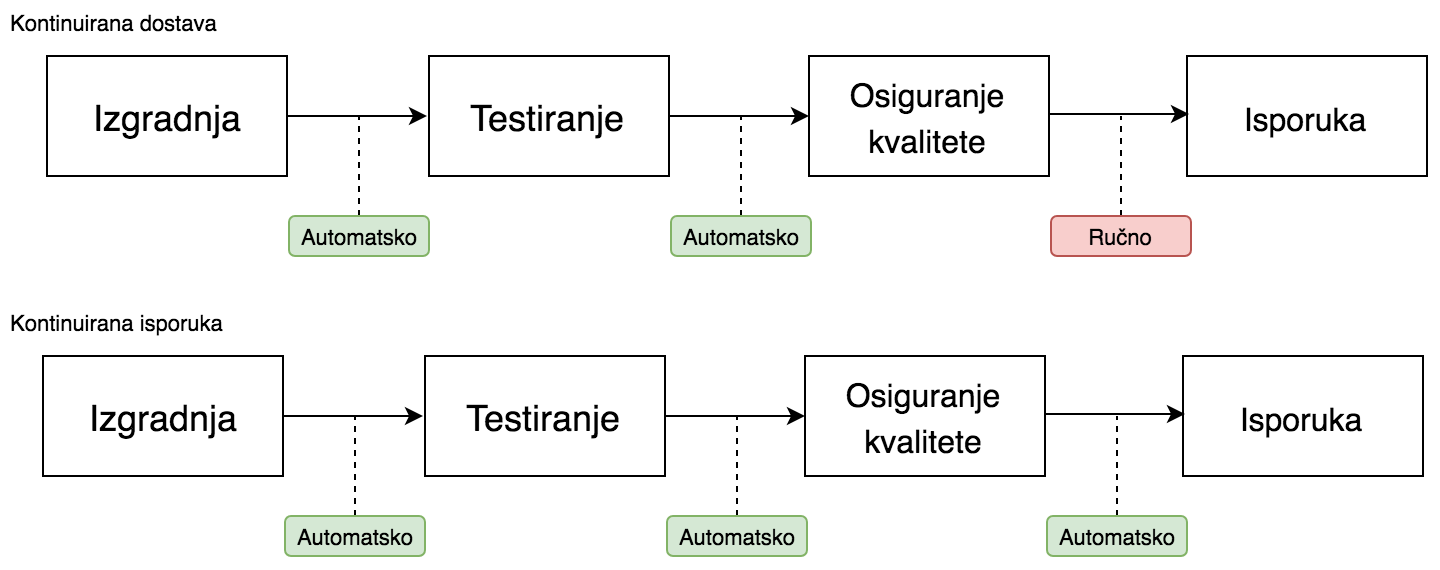
\includegraphics[scale=0.55]{CDDifferences}
\caption{Usporedba kontinuirane dostave i kontinuirane isporuke}
\label{fig:CDDifferences}
\end{figure}

Kontinuirana isporuka automatskom isporukom promjena u produkciju nastoji smanjiti vrijeme između razvoja funkcionalnosti i njene objave u produkciju te samim time ukupno vrijeme trajanja razvoja. Kontinuirana isporuka ova obavlja na dva načina. Prvo, automatizacijom isporuke i automatskom isporukom promjena, kontinuirana isporuka značajno smanjuje vrijeme koje tim mora uložiti za obavljanje isporuke. Druga stavka je direktna posljedica prve. Zbog smanjenja opterećenja koje isporuka nanosi na tim, obavljanje isporuke postaje puno lakše. Lakše obavljanje isporuke dovodi do češćeg obavljanja isporuke. Irska kompanije \textit{Intercom} u svom blogu bilježi stabilan porast broja dnevnih isporuka promjenu od produkcija. Od ispod 20 isporuka u 2012. godini, do preko 80 isporuka u 2015. godini. Slika \ref{fig:IntercomShipsPerDay} prikazuje broj dnevnih isporuka promjena u produkciju kompanije \textit{Intercom}\citep{intercom:cd}.

\begin{figure}
\centering
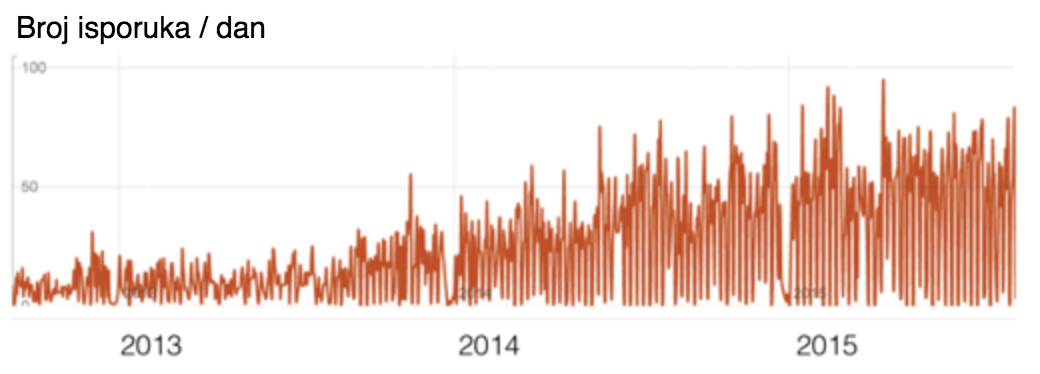
\includegraphics[scale=0.6]{IntercomShipsPerDay}
\caption{Broj dnevnih isporuka promjena u produkciju kompanije \textit{Intercom}}
\label{fig:IntercomShipsPerDay}
\end{figure}

Iako kontinuirana isporuka nastoji promjene automatski isporučiti u produkciju, navedeno ne znači da se svaka promjena koda automatski isporučuju direktno korisniku. Prvo, svaka promjena prolazi cijeli proces automatskog testiranja i provjere kvalitete. Dodatno, promjene u praksi često prolaze brojna ručna testiranja prije objave u produkciju. Ručna testiranja možemo generalno podijeliti na testiranja razvojnog tima, testiranja tima za osiguranje kvalitete i testiranja vanjskih korisnika koja po broju korisnika dijelimo na \textit{alpha} i |textit{beta} testove.

Dok se \textit{alpha} testiranja provode na vrlo malom broju korisnika, \textit{beta} testiranja mogu sadržavati i do 10% korisnika. Testiranja razvojnog tima provodi tim koji razvija aplikaciju. Ovi testovi nastoje potvrditi ispravnost razvijene funkcionalnosti ali ne ulaze dulje u ispravnost cijele programske podrške. Testiranja tima za osiguranje kvalitete nastoje osigurati ispravnost cijele programske podrške. Način, raspored i provođenje testiranja je strogo definiran te po opsegu daleko nadmašuje testiranje razvojnog tima. S druge strane, testiranja na vanjskim korisnicima ne provode zaposlenici već potencijalni budući korisnici. Korisnici ne testiraju programsku podršku već ju normalno koriste. Međutim, velik broj korisnika omogućava pronalazak i najmanje greške u programskoj podršci. Dodatno, ovaj tip testiranja se može iskoristiti i za praćenje ponašanja korisnika na temelju čega se mogu uvoditi poboljšanja produkta.

Umjesto da se programska podrška isporuči direktno korisnicima, ona prolazi niz ručnih testiranja. Primjer procesa isporuke produkta različitim skupinama korisnika je prikazana na slici \ref{fig:DeploymentStages}.

\begin{figure}[b]
\centering
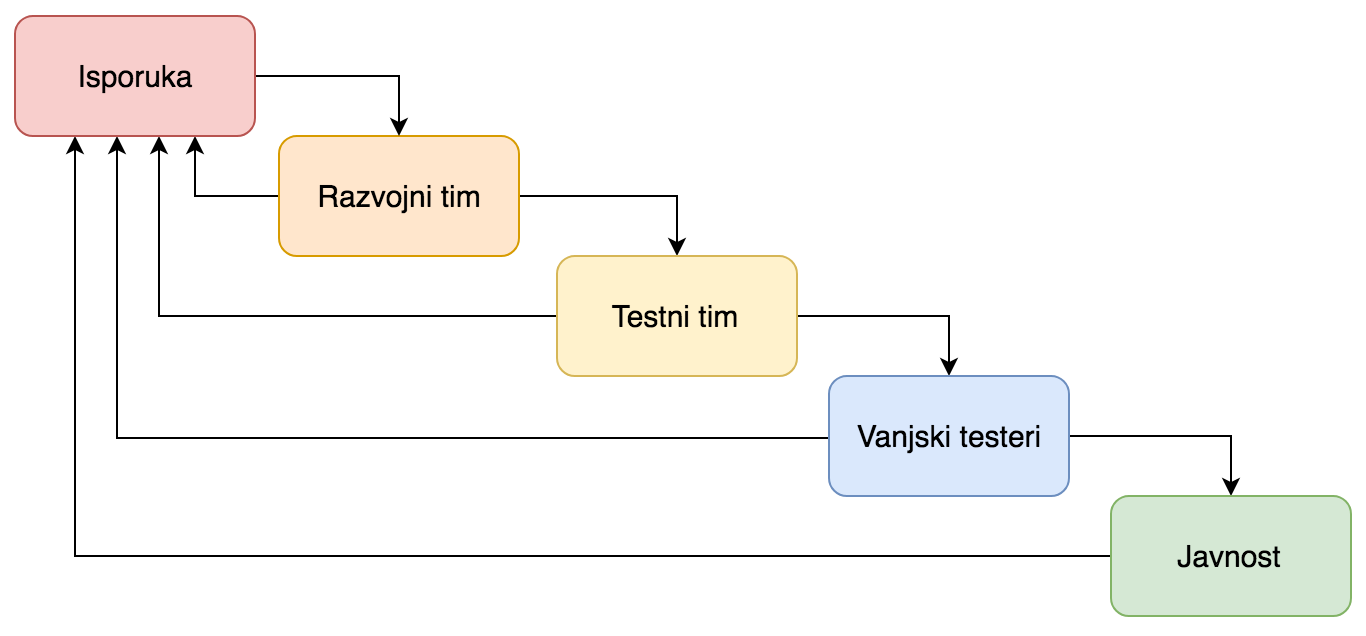
\includegraphics[scale=0.6]{DeploymentStages}
\caption{Postupna isporuka programske potpore skupovima korisnika}
\label{fig:DeploymentStages}
\end{figure}









\chapter{Zaključak}
Zaključak.

\bibliography{literatura}
\bibliographystyle{fer}

\begin{sazetak}
Sažetak na hrvatskom jeziku.

\kljucnerijeci{Ključne riječi, odvojene zarezima.}
\end{sazetak}

% TODO: Navedite naslov na engleskom jeziku.
\engtitle{Title}
\begin{abstract}
Abstract.

\keywords{Keywords.}
\end{abstract}




\begin{appendices}



\chapter{Ručna integracija i isporuka iOS aplikacija}

Ovaj dodatak je tehnički usmjeren pregled ručne implementacije procesa integracije i isporuke iOS aplikacije. Glavni cilj dodatka je upoznati se s alatima koje koristimo kod razvoja, integracije i isporuke iOS aplikacija. Sam postupak automatizacija donosi svoje prepreke, zbog čega je lakše prvo definirati postupak koji automatiziramo.

Prvi dio dodatka specificira alate koje koristim u razvoju, integraciji i isporuci te njihovu instalaciju i pripremu. Drugi dio obrađuje integraciju a treći isporuku.

Primjeri su napisani korištenjem operacijskog sustava \textit{macOS Sierra 10.12.4}.

\section{Alati} \label{AlatiBuild}

Sve naredbe su definirane za \textit{bash} ljusku. Ovoj ljusci je najjednostavnije pristupiti korištenjem \textit{termianl} aplikacije dostupne na svakoj instalaciji macOS operacijskog sustava. Naravno, moguće je koristiti bilo koji drugi tekstualno sučelje s pristupom bash ljusci.

Za provjeru postojanja alata koristim sljedeći naredbu. Naredbu ću koristiti za provjeru postojanja alata i izbjegavanje nepotrebne reinstalacije.

\begin{verbatim}
if which {ime_naredbe} >/dev/null; then
    echo "{ime_naredbe} installed"
else
    echo "{ime_naredbe} not installed"
fi
\end{verbatim}

Za razvoj iOS aplikacija koristim alat Xcode. Na tržištu postoji nekoliko sličnih alata, ali je Xcode daleko najpopularniji te ga koristimo i za ostvarenje automatizacije integracije. Alat je moguće instalirati korištenjem App Store aplikacije. Za testiranje procesa koje ću implementirati u ostatku ovog dodatka kreiram jednostavan testni projekt. Projekt je iOS aplikacija imena \textit{Diplomski\_rad} te sadrži jednu shemu istog imena. Projekt sadrži tri cilja: iOS aplikaciju, \textit{unit} i \textit{ui} testove.

\textit{Hombrew} je alat za instaliranje i upravljanje alatima za macOS operacijski sustav. Alat olakšava instalaciju i konfiguraciju nekoliko alata koje koristimo u sklopu razvoja. Mana ovog alata je zahtijevanje \textit{sudo} pristupa zbog čega instalaciju alata nije moguće automatizirati.

Homebrew je moguće preuzeti korištenjem sljedeće naredbe. Naredba prvo provjerava postojanje Homebrew aplikacije. Ako aplikacija ne postoji, onda ju preuzima sa službene stranice. Ako aplikacija postoji, onda naredba osvježava njeno stanje. Za dohvaćanje alata koristim naredbu \textit{ruby}. Navedena navedena naredba je prisutna na svim trenutnim instalacijama macOS operacijskog sustava.

\begin{verbatim}
if which brew >/dev/null; then
    brew update
else
    ruby -e "$(curl -fsSL https://raw.githubusercontent
        .com/Homebrew/install/master/install)"
fi
\end{verbatim}

Za upravljanje ovisnosti koristim alate CocoaPods i Carthage. Navedene alate dohvaćam respektivno naredbom pod (1) i naredbom pod (2). Naredba pod (1) osvježava postojeću instalaciju ako alat već postoji zbog čega ne provjeravam njegovo postojanje.

\begin{verbatim}
gem install cocoapods --user-install (1)

if ! which carthage >/dev/null; then
    brew install carthage (2)
fi
\end{verbatim}

\textit{Swiftlint} je alat za statičku analizu jezika Swift \eng{linting tool}. Alat je moguće preuzetim korištenjem Homebrew alata.

\begin{verbatim}
brew install swiftlint
\end{verbatim}


\section{Priprema} \label{IntegracijaDodatakA}

Integracija započinje verzioniranjem. U sklopu ovog rada koristim alat git a repozitorij objavljujem na Github stranici. Za kontrolu pristupa repozitoriju koristim \textit{ssh} protokol.

\subsection{Uvod u git} \label{uvodUGit}

Temeljne funkcionalnosti git alata su repozitoriji i grane. Repozitorij je direktorij koji je verzioniran korištenjem git sustava za kontrolu verzija. Ovaj repozitorij sadrži direktorij “.git” koji specificira na koji se način verzionira repozitori te sadrži informacije o repozitoriju.

Repozitoriji se mogu klonirati na istom ili drugom uređaju. Klonirani repozitorij je novi repozitorij koji sadržava svu povijest kloniranog repozitorija. Promjene koje se obavljaju u kloniranom repozitoriju nemaju nikakvog utjecaja na izvorni repozitorij. Međutim, promjene obavljene u kloniranom repozitoriju se mogu, uz postojanje odgovarajuće autorizacije, prenijeti na izvorni repozitorij. Prijenos promjena se ne mora obavljati isključivo između izvornog i kloniranog repozitorija, već se može obaviti između bilo koja dva povezana repozitorija.

\begin{figure}[b!]
\centering
\begin{minipage}{.5\textwidth}
\centering
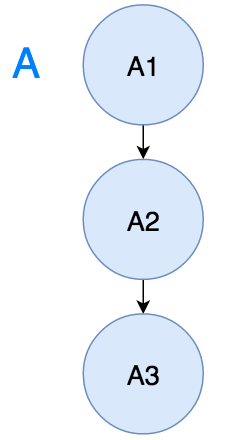
\includegraphics[scale=0.6]{Initial_commit}
\caption{Grana s tri potvrde}
\label{fig:Initial_commit}
\end{minipage}%
\begin{minipage}{.5\textwidth}
\centering
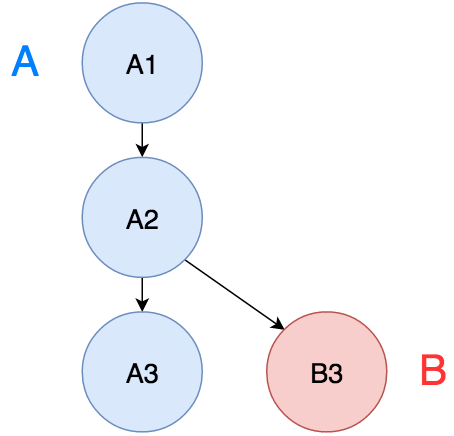
\includegraphics[scale=0.6]{Branching}
\caption{Grananje}
\label{fig:Branching}
\end{minipage}
\end{figure}

Prilikom kreiranja git repozitorija stvara se i glavna grana (eng. master branch) repozitorija. Grana je definirana slijedom promjena koje su primijenjene na njoj. Modificiranje dokumenata u repozitorija ne uzrokuje samo po sebi stvaranje nove verzije. Obavljene modifikacije je potrebno potvrditi \eng{commit}. Potvrđivanje modifikacija kreira novu verziju izvornog koda na trenutnoj grani te osvježava njeno stanje. Potvrđivanje promjena je prikazano na slici \ref{fig:Initial_commit}. Repozitorij koda se stvara kreiranjem glavne grane i obavljanjem inicijalnog potvrđivanja \eng{initial commit}. Glavna grana je označena slovom A. Inicijalno potvrđivanje je označeno s A1, dok su naknadna potvrđivanja označena s A2 i A3.

\begin{figure}
\centering
\begin{subfigure}{.49\textwidth}
\centering
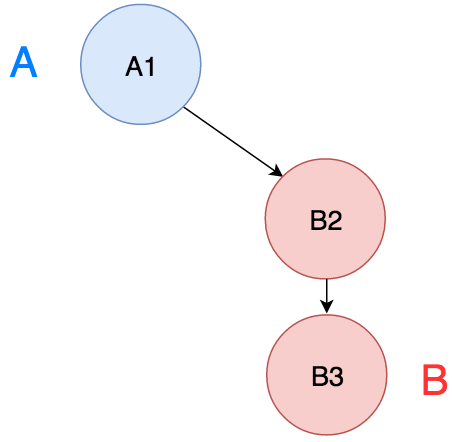
\includegraphics[scale=0.6]{FastForwardA}
\caption{Stanje prije spajanja}
\label{fig:FastForwardA}
\end{subfigure}
\begin{subfigure}{.49\textwidth}
\centering
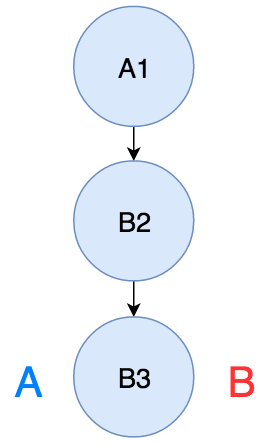
\includegraphics[scale=0.6]{FastForwardB}
\caption{Stanje nakon spajanja}
\label{fig:FastForwardB}
\end{subfigure}
\caption{Spajanja dodavanje promjena}
\label{fig:FastForward}
\end{figure}

Nova grana se može kreirati iz bilo kojeg stanja postojeće granje. Ovaj se postupak naziva grananje \eng{branching}. Izvorna i klonirana grana dijele zajedničku povijest do trenutka grananja. Daljnje promjene se primjenjuju samo na izvornu ili kloniranu granu. Slika \ref{fig:Branching} prikazuje postupak grananja. Grana B se kreira iz stanja A2 grane A. Grane A i B dijele dva zajednička stanja A1 i A2. Ova stanja nazivamo zajednička povijest grana. Nakon grananja na granu B dodajemo dva nova stanja B2 i B3.


\begin{figure}[b!]
\centering
\begin{subfigure}{.49\textwidth}
\centering
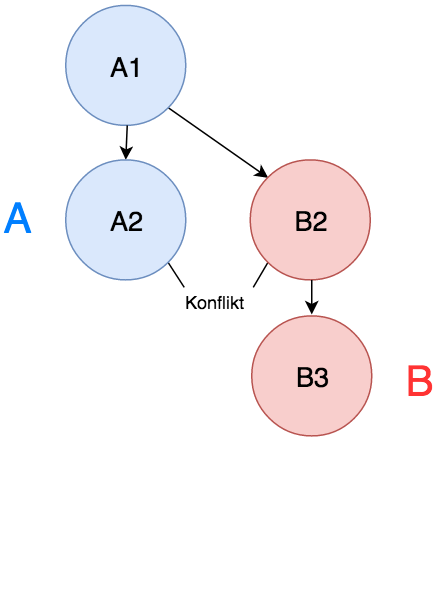
\includegraphics[scale=0.6]{ConflictA}
\caption{Stanje prije spajanja}
\label{fig:ConflictA}
\end{subfigure}
\begin{subfigure}{.49\textwidth}
\centering
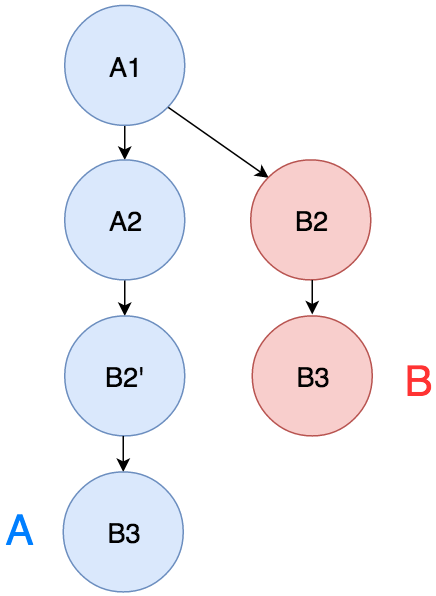
\includegraphics[scale=0.6]{ConflictB}
\caption{Stanje nakon spajanja}
\label{fig:ConflictB}
\end{subfigure}
\caption{Spajanja otklananjem konflikta}
\label{fig:Conflict}
\end{figure}

Grane je također moguće spojiti. Spajanje grana dodaje promjene obavljene na izvornoj \eng{source} grani u odredišnu \eng{destionation} granu. Spajanje je moguće obaviti na nekoliko načina ovisno o odnosu dviju grana koje se spajaju. Slika \ref{fig:FastForward} prikazuje najjednostavniji odnos dviju grana kod spajanja. Nakon grananja grane B iz stanja A2 grane A na granu B se dodaju dva nova stanja, B2 i B3. U međuvremenu je grana A ostala nepromijenjena. Zbog navedenog je spajanje grana moguće obaviti jednostavno dodavanjem promjena B grane na vrh A grane, \eng{fast forward}. Slike \ref{fig:FastForwardA} prikazuje stanje prije spajanja dok slika \ref{fig:FastForwardB} prikazuje stanje nakon spajanja. Dodatno, samo spajanje je moguće označiti dodavanjem dodatnog stanja na granu na kojoj se obavlja spajanje.

Postupak se komplicira ako je odredišna grana modificirana nakon grananja. U navedenom slučaju nije moguće promjene obavljene u izvorišnoj gani samo dodati na vrh odredišne grane, nego je promjene potrebno spojiti. Proces spajanja ovisi o tome postoje li konflikti između promjena. Ako ne postoji, spajanje je moguće obaviti jednako kao na slici \ref{fig:FastForward}, jednostavno dodavanjem promjena na vrh odredišne grane.

Međutim, ako promjene izazivaju konflikte, onda je te konflikte potrebno ručno razriješiti. Otklanjanje konflikata uzrokuje izmjenom verzija jedne ili obje grane. Proces otklanjanja konflikata se najčešće odrađuje dodavanjem jedne po jedne verzije izvorne grane na odredišnu granu. Ako dodana verzija ne izaziva konflikt, ona se jednostavno dodaje na vrh odredišne grane. Međutim, ako verzija izaziva konflikt, tada se isti otklanja modificirajući dodanu verziju. Slika \ref{fig:Conflict} prikazuje proces spajanja grana s konfliktom. Konflikt je nastao između verzija A2 i B2. Konflikt se otklanja dodavanjem verzije B2 na vrh A grane i njenim modificiranjem. Ovo je stanje označeno s B2'. Stanje B3 ne izaziva konflikt te se samo dodaje na vrh A grane. Rezultat spajanja su dvije grane A i B različitih povijesti.

\begin{figure}[h!]
\centering
\begin{subfigure}{.3\textwidth}
\centering
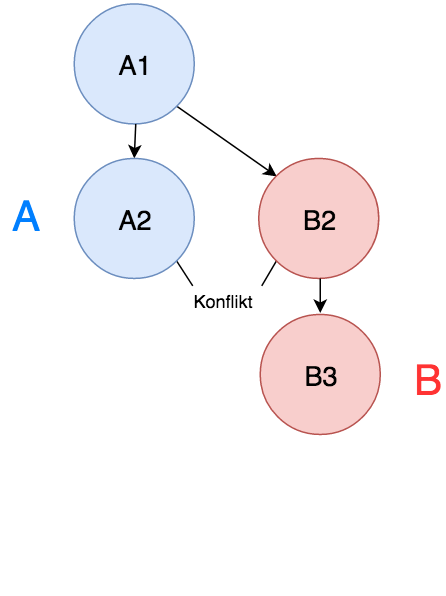
\includegraphics[scale=0.5]{RebaseA}
\caption{Početno stanje}
\label{fig:RebaseA}
\end{subfigure}
\begin{subfigure}{.3\textwidth}
\centering
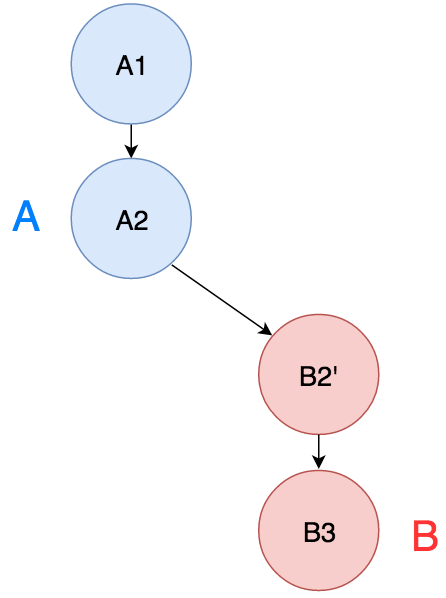
\includegraphics[scale=0.5]{RebaseB}
\caption{Stanje nakon \textit{rebase}}
\label{fig:RebaseB}
\end{subfigure}
\begin{subfigure}{.3\textwidth}
\centering
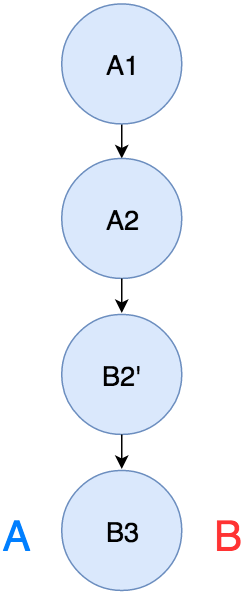
\includegraphics[scale=0.5]{RebaseC}
\caption{Stanje nakon spajanja}
\label{fig:RebaseC}
\end{subfigure}
\caption{Spajanje \textit{rebase} postupkom}
\label{fig:Rebase}
\end{figure}

Gore naveden slučaj se često rješava postupkom pod nazivom \textit{rebase}. Postupak prije spajanja u povijest izvorišne grane dodaje sve verzije nastala u odredišnoj grani nakon grananja. Verzije se dodaju odmah nakon stare točke grananja čime se točka grananja pomiče na zadnju verziju A grane. Slika \ref{fig:RebaseB} prikazuje stanje nakon obavljanja \textit{rebase} postupka na grani B. Sada su grane u stanju jednakom onom na slici \ref{fig:FastForward} te je spajanje moguće obaviti dodavanjem promjena na vrh odredišne grane. Stanje B2 se još uvijek mijenja, međutim sada je povijest repozitorija linearna.


\subsection{SSH ključ}

Novi ssh ključ se kreira naredbom u nastavku.

\begin{verbatim}
ssh-keygen -t rsa -b 4096 -C "email@primjer.com"
\end{verbatim}

Korisno je ključ dodati ssh agentu kako ne bi morali svaki put unositi šifru ključa.

\begin{verbatim}
eval "$(ssh-agent -s)"

ssh-add -K ~/.ssh/{ime_kljuca}
\end{verbatim}

Ključ je potrebno dodati na Github. Sljedeća naredba kopira javni dio ključa.

\begin{verbatim}
pbcopy < ~/.ssh/{ime_kljuca}.pub
\end{verbatim}


\subsection{Upravljanje ovisnostima}

Koristim dva alata za upravljanje ovisnostima - CocoaPods i Carthage. CocoaPods je stariji i široko prihvaćen alat za upravljanje ovisnostima iOS projekata. Alat je centraliziran. Ovisnosti moraju biti unaprijed registrirane na CocoaPods platformi zbog čega je složeno koristiti privatne ovisnosti i ovisnosti koje su još u razvoju. Carthage je noviji alat. Za razliku od CocoaPods alata, Carthage ne izmjenjuje datoteke projekta te je decentraliziran. Ovisnost nije potrebno registrirati te ih je moguće dohvatiti iz bilo kojeg repozitorija.

Kako bi osigurao ispravnost procesa dohvate ovisnosti, projektu dodajem četiri vanjske ovisnosti od kojih je jedna privatna.

\paragraph{CocoaPods}

CocoaPods alat se inicijalizira korištenjem naredbe u početnom direktoriju projekta.

\begin{verbatim}
pod init
\end{verbatim}

Ovisnosti se dodaju u novokreiranu datoteku \textit{Podfile}. Ovisnosti se dodaju željenom cilju. Ako su ciljevi ugniježđeni, onda se ovisnosti i postavke roditelja odnose i na djecu. Definiram dvije ovisnosti, \textit{LayoutKit} u glavnom cilju i \textit{Nimble} u testnom cilju. Sadržaj datoteke \textit{Podfile} je prikazan u nastavku.

\begin{verbatim}
use_frameworks!

target 'Diplomski_rad' do
  pod 'LayoutKit'
end


target 'Diplomski_radTests' do
  inherit! :search_paths
    pod 'Nimble'
end
\end{verbatim}

Ovisnosti se dohvaćaju naredbom:

\begin{verbatim}
pod install
\end{verbatim}

Naredba kreira novo radno okruženje pod imenom \textit{Diplomski\_rad.xcworkspace}. Radnom okruženju su dodana dva projekta: glavni projekt i novo kreirani \textit{Pods} projekt koji sadrži sve ovisnosti. Daljnji razvoj je potrebno nastaviti korištenjem kreiranog radnog okruženja.

\paragraph{Carthage}

Korištenjem alata Carthage također dohvaćam dvije ovisnosti ali je jedna od ovisnosti privatna ovisnost podignuta na privatnom \textit{gitlab} poslužitelju.

U početnom direktoriju repozitorija je potrebno kreirati datoteku pod nazivom \textit{Cartfile}. U datoteci se specificiraju sve javne ovisnosti. Privatne ovisnosti je moguće specificirati u \textit{Cartfile.private} datoteci. Sadržaj datoteke \textit{Cartfile} je prikazan u nastavku.

\begin{verbatim}
git "git@naziv_poslužitelja/ime_projekta.git" "ime_grane"

github "facebook/facebook-sdk-swift"
\end{verbatim}

Ovisnosti se dohvaćaju pokretanjem naredbe:

\begin{verbatim}
carthage update --platform ios
\end{verbatim}

Dohvaćene ovisnosti je potrebno ručno uključiti u projekt. Potrebno je odabrati željeni cilj te u \textit{General -> Linked Frameworks and Libraries} sekciju dovući željene biblioteke iz \verb|Carthage/Build| direktorija. U \textit{Build phases} sekciji dodati novu \textit{Run script} fazu s naredbom:

\begin{verbatim}
/usr/local/bin/carthage copy-frameworks
\end{verbatim}

U polje \textit{Input Files} dodati sve željene ovisnosti u obliku:

\begin{verbatim}
$(SRCROOT)/Carthage/Build/iOS/{ime_biblioteke}.framework
\end{verbatim}


\section{Integracija}

\subsection{Izgradnja} \label{IzgradnjeDodatak}

Za izgradnju, testiranje i arhiviranje iOS aplikacija koristim \textit{xcodebuild} alat. Alat je razvio Apple za izgradnju macOS aplikacija. U međuvremenu je alat proširen te danas podržava razvoj programske potpore za iOS, tvOS i watchOS operacijske sustave. Xcode i Xcode Server alati koriste xcodebuild za obavljanje svih operacija vezanih uz projekt. Iako se u procesu automatizacije nećemo direktno susretati s alatom, korisno je znati što se dešava u pozadini.

Alat je vrlo jednostavan za uporabu. Dovoljno je pokrenuti naredbu \verb|xcodebuild| u početnom direktoriju projekta. Ako u direktoriju postoji samo jedan projekt, naredba pokreće proces izgradnje za predodređenu shemu projekta.

Projekt i cilj se je moguće odabrati korištenjem sljedećih parametara:

\begin{verbatim}
xcodebuild [-project imeprojekta] [-target imecilja]
\end{verbatim}

Shema projekta se odabire \verb|scheme| parametrom:

\begin{verbatim}
xcodebuild [-project imeprojekta] -scheme imesheme
\end{verbatim}

Naredba prima operaciju kao argument. Ako operacija nije specificirana, xcodebuild naredba predodređeno pokreće izgradnju \eng{build}. Ostale podržane operacije su:

\verb|analyze| - Izgrađuje i analizira cilj ili shemu

\verb|archive| - Arhivira i priprema projekt za objavu

\verb|test| - Izgrađuje i testira shemu

\verb|installsrc| - Kopira izvorni kod u \verb|SRCROOT|

\verb|install| - Izgrađuje i instalira projekt u ciljni direktorij projekta \verb|DSTROOT|

\verb|clean| - Briše metapodatke i rezultate izgradnje

Ispis xcodebuild operacije je vrlo detaljan. Operacija ispisuje sve postupke koje obavlja te daje detaljno izvješće u slučaju pogreške. Međutim, ovaj tip ispisa je teško čitljiv. Zbog navedenog se često koriste alati koji parsiraju i prikazuju ispis u lakše čitljivom formatu.

\subsection{Testiranje} \label{TestiranjeXcodeBuild}

Xcode projekt implementira dvije vrste testova: \textit{Unit} i \textit{UI} testove. Oba tipa testa su implementirani kao ciljevi unutar projekta koji pokazuju na cilj aplikacije. Unit testovi služe za testiranje unutarnje implementacije projekta. Ovaj tip testa se pokreće kao omotač oko izvorne aplikacije te pristupa njenim resursima. UI test omogućava testiranje ponašanja aplikacije u stvarnom svijetu. Navedeni tip testa simulira korisničku interakciju te provjerava ponašanje aplikacije.

Oba tipa testa se pokreću na iOS simulatoru. Zbog navedenog je potrebno imati barem jedan simulator prihvatljive verzije operacijskog sustava. Simulatore je moguće dohvatiti pomoću Xcode alata. Za prikaz dostupnih simulatora je moguće iskoristiti naredbu:

\begin{verbatim}
instruments -s devices
\end{verbatim}

Testiranje se pokreće naredbom:

\begin{verbatim}
xcodebuild test -workspace Diplomski_rad.xcworkspace
    -scheme Diplomski_rad
    -destination 'platform=iOS Simulator,OS=10.3,
    name=iPhone 7'
\end{verbatim}

Naredba će pokrenuti testni cilj odabrane sheme na odabranom radnom okruženju. Odabir drugog projekta, cilja i sheme se radi jednako kao i kod izgradnje. Za pokretanje drugog testnog cilja je potrebno kreirati novu shemu te joj kao cilj testne operacije postaviti željeni testni cilj.

\subsection{Osiguranje kvalitete} \label{OsiguranjeKvaliteteImplementacija}

U sklopu osiguranja kvalitete provodim dva procesa: provjeru pokrivenosti koda testovima i statičku provjeru koda alatom \textit{Swiftlint}.

Provjeru pokrivenosti koda dobivamo koristeći parametar \verb|-showBuildSettings| pri izgradnji i testiranju projekta. Primjer naredbe:

\begin{verbatim}
xcodebuild -workspace Diplomski_rad.xcworkspace
    -scheme Diplomski_rad -showBuildSettings
\end{verbatim}

Naredba podatke o pokrivenosti koda sprema u \verb|~/Library/Developer/|\\\verb|Xcode/DerivedData/{ime_projekta+slučajan_identifikator}/|\\\verb|Build/Intermediates/CodeCoverage| direktoriju. Generirani dokumenti su teško čitljivi. Postoji nekoliko alata koji ih obrađuju i generiraju čitljive rezultati. Budući da u razvoju koristim Xcode, neću u njih dublje ulaziti.

Switlint je alat za statičku analizu koda napisanog u programskom jeziku Swift. Alat definira veliki broj pravila kojim nastoji osigurati praćenje stila i konvencija jezika Swift. Većina pravila se odnosi na izgled i format koda, ali postoje i pravila koja nastoje izbjeći pojavu grešaka.

Alat se pokreće pozivanjem naredbe \verb|swiftlint| u početnom direktoriju projekta. Ispis alata je sličan onome xcodebuild alata. Za lakše praćenje pogrešaka i pokretanje naredbe kod svakog procesa izgradnje je moguće Xcode projektu dodati novu \verb|Run Script| fazu s naredbom:

\begin{verbatim}
if which swiftlint >/dev/null; then
    swiftlint
else
    echo "warning: Swiftlint nije instaliran"
fi
\end{verbatim}



\section{Isporuka} \label{header:ImplementacijaIsporuke}

Kao što je navedeno u odlomku \ref{header:RucnaIsporuka}, isporuka programske potpore za iOS operacijske sustave dolazi u četiri tipa: direktna isporuka, \textit{ad hoc} isporuka , unutarnja isporuka i isporuka korištenjem App Store platforme. U nastavku je prikazana ručna implementacija svakog tipa.

Direktna isporuka aplikaciju instalira na mobilni uređaj koji je direktno povezan s računalom koje obavlja isporuku. Uređaj je prije isporuke potrebno registrirati kao testni uređaj na Apple developer računu. Za pristup Apple Developer računu se je potrebno u isti prijaviti na \verb|https://developer.apple.com/| stranici. Nakon prijave odabrati opciju \verb|Certificates, Identifiers & Profiles|. U lijevom bočnom izborniku odabrati opciju \verb|Devices| te u gornjem desnom kutu klikom na \textit{plus} ikonu pokrenuti proces registriranja novog testnog uređaja. Za registraciju je potrebno dohvatiti UUID uređaja. UUID se može dohvatiti korištenjem iTunes aplikacije dostupne na macOS operacijskom sustavu. Potrebno je povezati mobilni uređaj s računalom korištenjem USB kabla. U iTunes aplikaciji odabrati povezani mobilni uređaj te kopirati UUID uređaja. Slika \ref{fig:iTunesUUID} prikazuje lokaciju UUID broja u iTunes aplikacije.

\begin{figure}
\centering
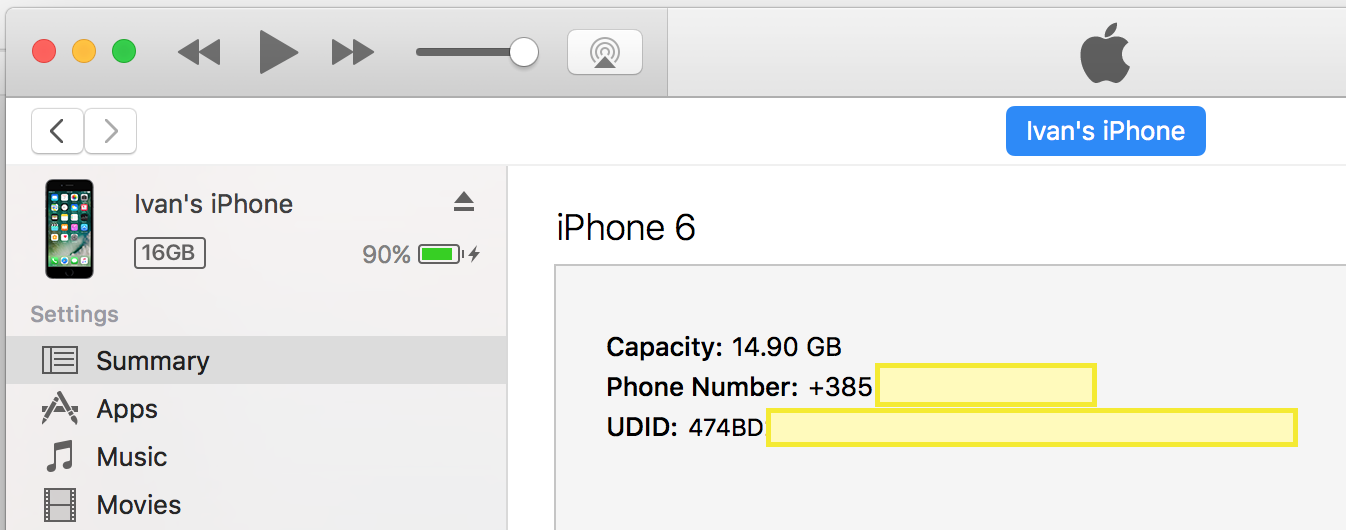
\includegraphics[scale=0.5]{iTunesUUID}
\caption{Dohvat UUIDa uređaja korištenjem iTunes aplikacije}
\label{fig:iTunesUUID}
\end{figure}

Nakon dohvata UUIDa je isti potrebno kopirati u formu za registriranje testnog uređaja.

Dodatno, prije isporuke aplikacije je potrebno kreirati certifikat za razvoj i certifikat za osobu koja obavlja isporuku. Svaki certifikat se sastoji od privatnog i javnog dijela. Javan dio je slobodno dijeliti te se uvijek može preuzeti s Apple Developer računa. S druge strane, tajni dio certifikata se mora održati strogo tajnim te instalirati samo na uređajima koji zahtijevaju navedeni certifikat. Proces kreiranja i održavanja certifikata je poprilično komplicirao proces razvoja i isporuke. Zbog navedenog je Apple ugradio podršku za automatsko upravljanje certifikatima. Ovim postupkom je gotovo u potpunosti eliminirana potreba ručnog kreiranja i održavanja certifikata. Za uključenje opcije je potrebno odabrati \verb|Automatically manage signing| opciju na željenom cilju projekta.

Certifikate je moguće kreirati ručno korištenjem Apple Developer platforme. Proces je sličan registraciji testnog uređaja. Nakon prijave potrebno je odabrati opciju \verb|Certificates, Identifiers & Profiles -> Identifiers|. Kreiranje certifikata je dobro definirano te je potrebno samo slijediti uputstva.

Instalaciju aplikacije na uređaj ostvarujem korištenjem Xcode alata. Potrebno je odabrati željeni spojen uređaj i pokrenuti \verb|run| operaciju na željenoj shemi. Operacija izgrađuje i instalira aplikaciju na odabranom uređaju. Apple zbog sigurnosnih razloga drži tajnim proces isporuke aplikacije na uređaj zbog čega je navedeni proces moguće ostvariti samo korištenjem Xcode alata.

Implementacija ad hoc i unutarnje isporuke je vrlo slična. Procesi se razlikuju u certifikatima koje koriste i u tome da ad hoc isporuka zahtijeva prethodnu registraciju testnog uređaja. Proces isporuke započinje arhiviranjem aplikacije. Arhiviranje aplikacije je moguće ostvariti korištenjem alata xcodebuild uz specificiranje \verb|archive| operacije i željene sheme. Navedena operacija prvo izgrađuje projekt uz korištenje opcija optimizacije. Primjer naredbe je prikazan u nastavku.

\begin{verbatim}
xcodebuild -scheme {imesheme} archive
\end{verbatim}

Naredba je interaktivna te od korisnika zahtijeva unos nekoliko parametara. Dovoljno je slijediti upute naredbe. Naredba generira dvije datoteke. Arhivu aplikacije s \verb|.ipa| nastavkom i manifest aplikacije s \verb|.plist| nastavkom. Arhiva aplikacije se koristi za instalaciju aplikacije na mobilni uređaj, dok se manifest može koristiti za jednostavnije preuzimanje arhive. Unutar manifesta je moguće specificirati lokaciju arhive. Budući da je manifest vrlo mala xml datoteka, jednostavno ju je moguće podijeliti sa svim potrebnim osobama. Na temelju preuzetog manifesta sustav preuzima povezanu arhivu i instalira aplikaciju.

Arhivu i manifest je moguće objaviti na nekoliko načina. Osnovan način je korištenjem vlastitog poslužitelja distribuirati potrebne datoteke. Najjednostavnije je napraviti jednostavnu HTML stranicu koja sadrži poveznicu na manifest. Manifest je moguće distribuirati i korištenjem drugih metoda dijeljena kao što su email ili Dropbox, ali je arhivu potrebno objaviti na poslužitelju.

Sljedeći način objave koristi službeni Appleov alat \textit{Mobile Device Management, MDM}. Alat je namijenjen za jednostavnu isporuku i distribuciji aplikacija koje nisu namijenjene za javnu objavu. Po funkcionalnosti je vrlo sličan App Store platformi. MDM omogućava jednostavnu objavu aplikacije i novih verzija te omogućava automatsku izgradnju i osvježenje verzije aplikacije. Međutim, alat je vrlo skup te ga koriste gotovo isključivo velike kompanije.

Danas je na tržištu dostupan veliki broj alata koji implementiraju funkcionalnosti slične MDMu za značajno manju cijenu. Najpopularniji od ovih alata je alat Crashlytics. Kompanija je osnovana 2011 godine s ciljem praćenja i dojave pogreška i rušenja mobilnih aplikacija. Kompaniju je 2013 godine kupio Twitter a početkom 2017 kupio Google. Danas alat uz praćenje pogrešaka olakšava distribuciju aplikacija i automatizaciju procesa.

Isporuka aplikacija pomoću Crashlytics alata je vrlo jednostavna. Potrebno je samo registrirati aplikaciju i dodati arhivu. Svi korisnici kojima je aplikacija vidljiva ju mogu jednostavno preuzeti i instalirati na uređaj. Alat je detaljnije obrađen u poglavlju \ref{header:KontinuiranaDostavaAutomatizacija} gdje ga koristim za automatizaciju procesa isporuke.

Za objavu javnih aplikacija je isporuku potrebno obaviti korištenjem App Store platforme. Objava aplikacija na App Store platformu se obavlja korištenjem iTunes Connect alata. Za pristup alatu je potrebno posjedovati Apple Developer račun. Proces započinje arhiviranjem aplikacije i registracijom iste korištenjem iTunes Connect alata.

Nakon prijave u \verb|https://itunesconnect.apple.com/| stranicu potrebno je odabrati opciju \verb|Apps|. Proces registracije aplikacije je poprilično jednostavno pratiti. Prvo je potrebno specificirati osnovne informacije o aplikaciji kao što su ime, opis i kategorija aplikacije. Nakon toga je potrebno dostaviti sve potrebne grafike koje uključuju nekoliko verzija ikone aplikacije koja je prikazana na početnom ekranu uređaja te slike potrebne za App Store platformu. Na kraju je potrebno dostaviti konačnu verziju aplikacije i time započeti proces provjere aplikacije. Ako proces završi uspješno aplikacija se izdaje na App Store platformu. U suprotnom je potrebno razriješiti razlog odbijanja aplikacije ponovno započeti proces provjere.



\chapter{Xcode Server} \label{XcodeServer}

Za automatizaciju procesa navedenih u odlomku A koristim alat Xcode Server. Na tržištu postoji veliki broj alata koji omogućuju automatizaciju procesa integracije. Razlog odabira alata Xcode Server objašnjavam u dodatku \ref{UsporedbaCIAlata_DodatakC}.

\section{Priprema} \label{PripremaAlata}

MacOS je, s ciljem sigurnosti, vrlo zatvorena platforma. Brojni alati zahtijevaju \verb|sudo| lozinku, korisničku interakciju te ih nije moguće instalirati korištenjem ljuske. Zbog navedenog instalaciju ovih alata nije moguće automatizirati već oni moraju biti unaprijed instalirani na računalu. Među njima su macOS Server, Xcode i Homebrew alati.

\begin{verbatim}
su - xcodeserver

export PATH=$PATH:/usr/local:~/.gem/ruby/2.0.0/bin
\end{verbatim}

Za dohvat brojnih alata koristim \textit{Homebrew} alat. Instalacija alata zahtijeva korištenje računa s administracijskim pravima \eng{sudo user}. Budući da novokreirani račun nije administrator, proces instalacije je potrebno obaviti na računu koji posjeduje navedena prava. Nakon instalacije je potrebno Xcode Server računu omogućiti korištenje alata i dati pristup \verb|/usr/local| direktoriju u kojem Homebrew obavlja izmjene. Naredba pod (1) instalira alat Homberew, naredba pod (2) kreira \verb|ci| grupu, naredba pod (3) dodaje trenutni i Xcode Server račun grupi, dok (4) daje potrebna prava grupi.

\begin{verbatim}
/usr/bin/ruby -e "$(curl -fsSL https://raw.githubuser
    content.com/Homebrew/install/master/install)" (1)

sudo dseditgroup -o create ci (2)

sudo dseditgroup -o edit -a {current_user} -t user ci (3)
sudo dseditgroup -o edit -a xcodeserver -t user ci

sudo chgrp -R ci /usr/local (4)
sudo chmod -R g+wr /usr/local
\end{verbatim}

\section{Kontinuirana integracija} \label{KontinuiranaIntegracija_DodatakB}

Kreiranje, konfiguraciju i praćenje automatiziranih procesa obavljam korištenjem alata Xcode. Procesi se pokreću i izvršavaju na macOS Serveru. Računalo na kojem se nalazi macOS Server se naziva poslužitelj. MacOS Serveru je moguće pristupiti korištenjem proizvoljnog Xcode alata, sve dok je server vidljiv te postoje odgovarajuća prava pristupa. Za spajanje na udaljeni macOS Server je potrebno pokrenuti lokalan macOS Server i u ponuđenim opcijama odabrati udaljeni poslužitelj.

Automatizacija Xcode procesa se ostvaruje korištenjem \textit{bota}. Bot je namijenjen specifično za automatizaciju Xcode projekata te je kreiranje i konfiguriranje kontinuirane integracije jednostavna u usporedbi s drugim alatima.

Bot se kreira korištenjem Xocde alata, \textit{Product -> Create bot...}. Potrebno je imenovati bot i odabrati macOS Server na kojem će se bot izvršavati.

Bot je potrebno povezati s repozitorijem izvornog koda. Ova veza omogućava pokretanje integracije nakon izmjene stanja repozitorija. Moguće je koristiti lokalno ili javno hostani repozitorij verzioniran alatom git ili svn.

Nakon povezivanja s repozitorijem izvornog koda je moguće konfigurirati opcije integracije. Moguće je odabrati željenu shemu te operacije koje će se izvršavati. Shema mora biti javna da bi se mogla automatizirati. Opcije su prikazane na slici \ref{fig:XcodeServerOptions}. Testove je moguće obaviti na iOS simulatoru i na stvarnim uređajima povezanim sa serverom.

\begin{figure}[h!]
    \centering
    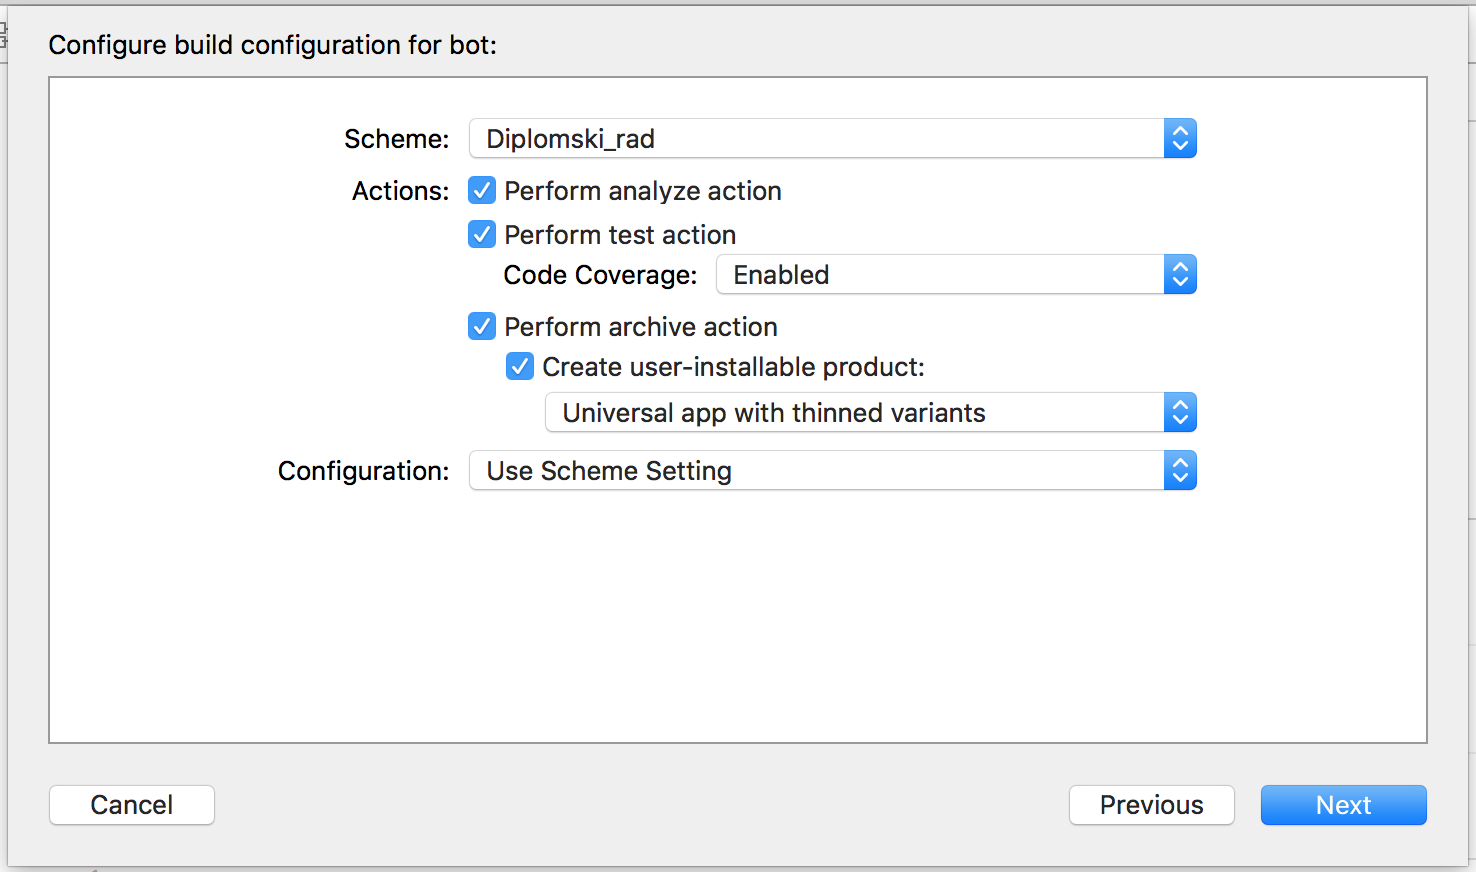
\includegraphics[scale=0.5]{XcodeServerOptions}
    \caption{Konfiguracija osnovnih opcija integracije}
    \label{fig:XcodeServerOptions}
\end{figure}

Integraciju je moguće pokretati periodički, nakon promijene stanja ili ručno.

\begin{figure}
    \centering
    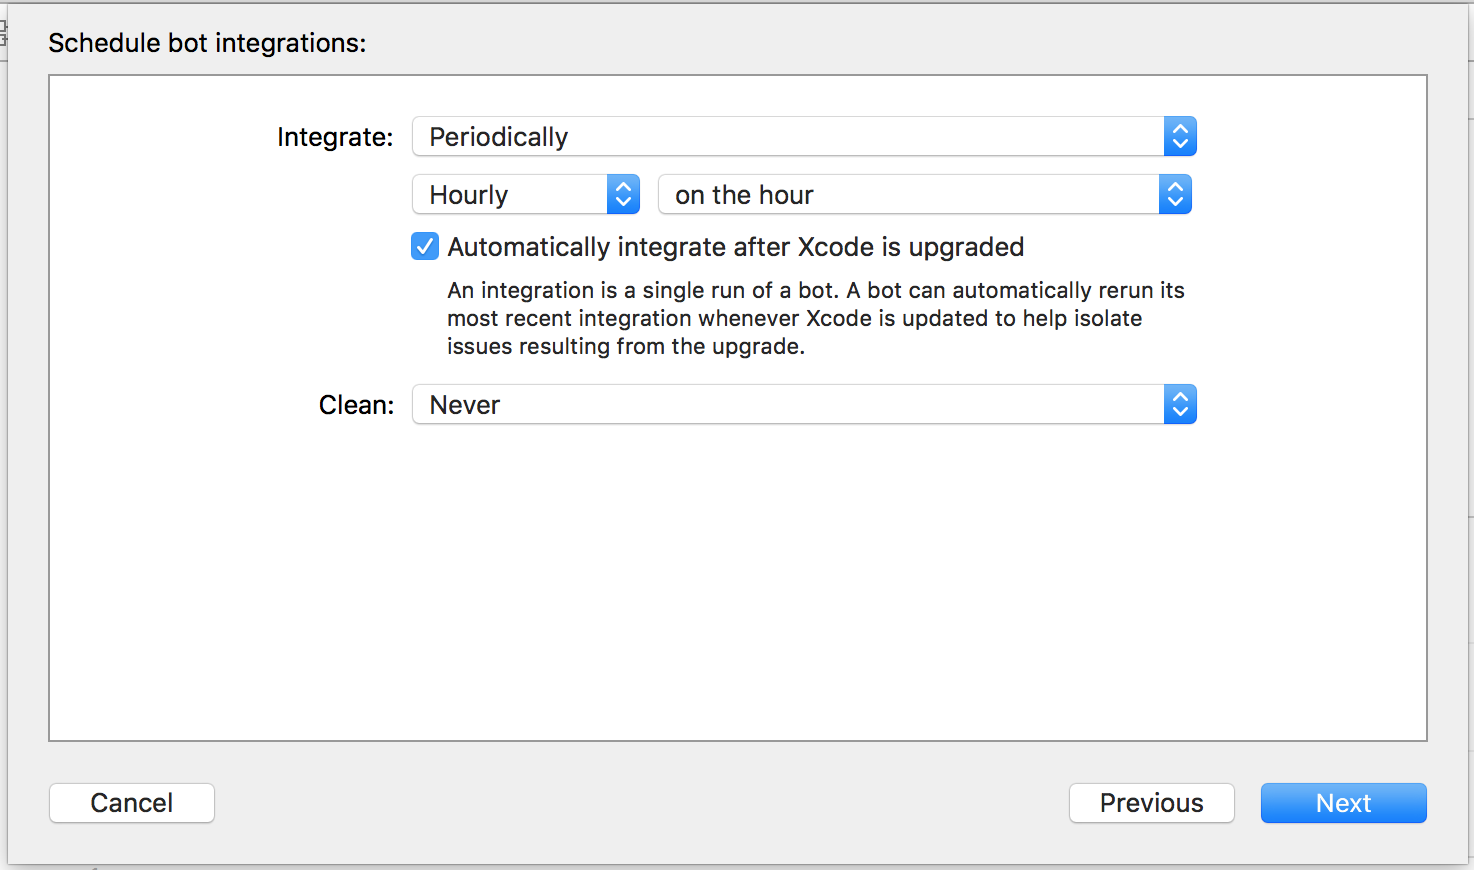
\includegraphics[scale=0.5]{XcodeServerIntegrationPeriods}
    \caption{Konfiguracija perioda izvršavanja integracije}
    \label{fig:XcodeServerIntegrationPeriods}
\end{figure}

Dodatno, moguće je konfigurirati okolinu u kojoj će se integracija izvršavati te pomoću \textit|sh| ljuske specificirati akcije koje se obavljaju prije i poslije obavljana integracije. Okolina se konfigurira postavljanjem proizvoljnog broja ključ - vrijednost parova. Akcije su proizvoljne skripte definirane i pokrenute na \textit{bin/sh} ljusci. Obje funkcionalnosti se ekstenzivno koriste za ostvarenje kontinuirane dostave i isporuke.

Integracija započinje odmah nakon kreiranja bota. Proces je moguće ručno započeti odabirom \textit{Integrate} opcije u gornjem desnom kutu.

Prva integracija završava pogreškom koju izaziva ne postojanje potrebnih ovisnosti. Xcode Server kreira privatnu verziju repozitorija izvornog koda te na njemu obavlja integraciju. Problem ovisnosti je moguće riješiti na dva načina.

Sve potrebne ovisnosti je moguće dodati repozitoriju izvornog koda. Korištenjem navedenog postupka su sve ovisnosti prisutne u repozitoriju odmah nakon preuzimanja repozitorija zbog čega ih nije potrebno dohvaćati. Navedeni postupak olakšava i ubrzava proces integracije. Međutim, dodavanje svih ovisnosti u izvorni repozitorij nosi i značajne probleme. Prvo, repozitorij koda postaje poprilično veći. Pregledom vlastitih projekata ustanovio sam da su ovisnosti od 2 do 50 puta veće od projekta. Čak su i u najvećem projektu ovisnosti bile značajno. Povećanje repozitorija usporava preuzimanje i otežava praćenje promjena. Iako navedeni postupak ima svojih prednosti, generalno se izbjegava u praksi.

Drugi pristup je potrebne ovisnosti specificirati u izvornom repozitoriju te ih dohvatiti po potrebi. Ovaj proces je vremenski zathjevniji od prošlog. Dohvaćanje i ponovna izgradnja svih ovisnosti može značajno usporiti proces integracije. Zbog navedenog je vrlo važno dohvaćati samo potrebne ovisnosti. Ostvarivanje optimalnog ponašanja značajno ovisi o alatu koji koristimo.

Implementacija prvog pristupa je vrlo jednostavna. Potrebno je sve ovisnosti dodati u repozitorij, odnosno maknuti ih iz \textit{.gitignore} dokumenta.

Implementacija drugog pristupa je nešto složenija. Za upravljanje ovisnostima u iOS razvoju se koriste dva alata: CocoaPods i Carthage. Oba alata imaju svoje prednosti i mane zbog čega demonstriram korištenje oba. Detaljan opis oba alata i razlog njihova korištenja se nalazi u dodatku A.

\subsection{CocoaPods}

Instalaciju CocoaPods možemo automatizirati korištenjem akcije koja se ostvaruje u sklopu integracije. Akcije se botu dodaju odabirom opcije \verb|Edit bot -> Triggers| te pritiskom na \textit{plus} ikonu u doljnem lijevom kutu. Moguće je kreirati akcije koje se izvršavaju prije ili poslije integracije. U ovom slučaju odabrati akciju koja se izvršava prije integracije te joj dodati naredbu u nastavku.

\begin{verbatim}
if which pod >/dev/null; then
    echo "CocoaPods found"
else
    echo "CocoaPods not found, proceeding with installation"

    if which gem >/dev/null; then
        gem install cocoapods --user-install

        pod repo update
    else
        echo "gem not found, quiting CocoaPods instalation"
    fi
fi
\end{verbatim}

U slučaju ne postojanja CocoaPods alata, naredba ga instalira i konfigurira. Za instalaciju CocoaPods alata koristim \verb|gem| alat koji je dostupan na svim instalacijama macOS operacijskog sustava. U slučaju promjene lokacije alata je istu potrebno izmijeniti u naredbi. Naredba pod (1) dohvaća i instalira CocoaPods alat. Naredba pod (2) dodaje direktorij u kom se nalazi CocoaPods alat u \verb|PATH| varijablu.

CocoaPods ovisnosti definira u \verb|Podfile| dokumentu. Za dohvaćanje i pripremu ovisnosti je dovoljno pozvati naredbu \verb|pod install|. Naredba dohvaća specifičnu verziju ovisnosti definiranu u \verb|Pofile.lock| datoteci. Ako ovisnost odgovarajuće verzije već postoji u lokalnom repozitoriju onda se ista ne dohvaća ponovno.

\begin{verbatim}
if [ -f Podfile ]; then
    pod install
fi
\end{verbatim}


\subsection{Carthage}

Za instalaciju Carthage alata koristim Homebrew alat. Proces je sličan instalaciji CocoaPods alata.

\begin{verbatim}
if which carthage >/dev/null; then
    echo "Carthage found"
else
    echo "Carthage not found, proceeding with installation"

    if which brew >/dev/null; then
        brew install carthage
    else
        echo "Homebrew needs to be installed"
    fi
fi
\end{verbatim}

Carthage ovisnosti specificira u Cartfile datoteci. Ako datoteka postoji u direktoriju, ovisnosti se mogu dohvatiti pozivajući \verb|carthage update| naredbu. Za bolje performanse operacije koristim dva argumenta. Argument \verb|--platform ios| specificira dohvaćanje ovisnosti samo za iOS platformu. Argument \verb|--cache-builds| dohvaća ovisnosti samo ako iste nisu već dostupne.

\begin{verbatim}
if [ -f Cartfile ]; then
    echo "Fetching dependencies using Carthage"

    carthage update --platform ios --cache-builds
else
    echo "Skipped fetching dependencies using Carthage"
fi
\end{verbatim}

Nakon dodavanja navedene četiri naredbe kao akcije koje se izvršavaju prije integracije projekt bi se trebao uspješno izgraditi. Ispis procesa koje obavlja integracija se nalazi u \verb|Logs| sekciji bota. U slučaju postojanja pogreške korisno je pogledati ispis procesa.

\subsection{Testiranje i osiguranje kvalitete}

Testovi se pokreću odabirom sheme koja za testnu operaciju koristi željene testne ciljeve i uključivanjem opcije \verb|Perform test action| u postavkama integracije. Predodređeno shema za testove pokreće oba testna cilja (UI i Unit) testove. Za isključivanje pojedinog testnog cilja ili dodavanje novih je potrebno modificirati testne postavke sheme.

Prikupljanje podatka o pokrivenosti koda testovima se uključuje odabirom opcije \verb|Code Coverage -> Enabled| u postavkama integracije.

Ako je poziv \verb|swiftlint| naredbe dodan kao \verb|Run script| faza u projektu, onda se isti poziva prilikom svake izgradnje i nije potrebno obavljati nikakve modifikacije. Ispis naredbe se parsira zajedno s ispisom xcodebuild alata te se rezultati dojavljuju zajedno. Ako naredba nije dodana projektu onda je poziv potrebno ručno implementirati nakon obavljanja integracije. Kod korištenja ovog pristupa je potrebno ispis samostalno parsirati.

Rezultate integracije je moguće vodjeti odabirom željenog bota korištenjem Xcode alata. Primjer rezultata je prikazan na slici \ref{fig:XcodeServerResult}.

\begin{figure}
    \centering
    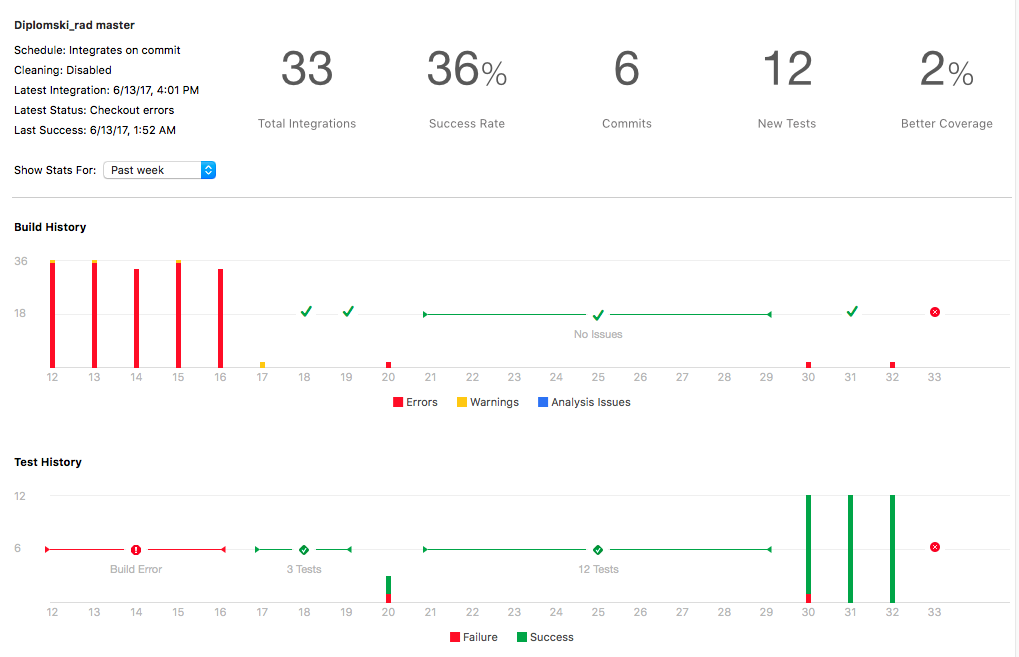
\includegraphics[scale=0.4]{XcodeServerResult}
    \caption{Rezultati procesa integracije}
    \label{fig:XcodeServerResult}
\end{figure}

\section{Kontinuirana dostava} \label{header:KontinuiranaDostavaAutomatizacija}



\chapter{Fastlane}

Automatizaciju isporuke programske potpore za iOS operacijski sustav obavljam pomoću alat fastlane. Danas je alat dio Fabric familije koju je u siječnju 2017. godine kupio Google. Fastlane je kolekcija manjih alata od kojih je svaki zadužen za automatizaciju pojedine operacije. Ove alate nazivamo dodaci. Većina dodataka je razvijena od strane zajednice te se kontinuirano razvijaju novi dodaci. Fastlane specificira i jednostavan način ulančavanja i pokretanja dodataka što značajno olakšava automatizaciju. Iako fastlane koristim samo za automatizaciju isporuke, alat podržava i automatizaciju ostalih operacija kao što su izgradnja i testiranje\citep{fastlane}.

Instalaciju alata obavljam koristeći Homebrew. Naredba je prikazana u nastavku.

\begin{verbatim}
brew cask install fastlane
\end{verbatim}

Inicijalizacija fastlane alata se obavlja pozivajući naredbu \verb|fastlane init| u početnom direktoriju projekta. Naredba kreira novi direktorij imena \verb|fastlane| te unutar njega stvara dvije tekstualne datoteke: \verb|Fastfile| i \verb|Appfile|.

Fastfile datoteka olakšava uporabu fastlane alata. Unutar datoteke je moguće definirati staze \eng{lane}. Svaka staza je sastavljena od proizvoljnog broja naredaba koje se izvršavaju slijedno. Dodatno, moguće je definirati naredbe koji se izvršavaju prije ili poslije željenih staza. Prilikom inicijalizacije alat fastlane detektira postavke projekta te na temelju njih stvara nekoliko predodređenih staza. Na primjer, ako projekt sadrži testni cilj, onda fastlane u Fastfile dokumentu kreira testnu stazu. Ako projekt sadrži Cartfile ili Podfile datoteku, onda fastlane dodaje pozive respektivno carthage ili cocoapods dodataka.

Primjer staze je prikazan u nastavku.

\begin{verbatim}
lane :{imestaze} do
    {naredbe}
end
\end{verbatim}

Pokretanje staze se obavlja pozivanjem naredbe \verb|fastlane {imestaze}| u početnom direktoriju projekta.

Appfile sadrži postavke projekta kao što su korisničko ime i id Apple Developer računa, korisničko ime i ime projekta na Crashlytics platformi te druge varijable koje se koriste u automatizaciji procesa.

Uz zavedene datoteke, fastlane direktorij može sadržavati i brojne druge tekstualne dokumente koji specificiraju postavke pojedinog dodatka. Datoteke slijede istu shemu imenovanja. Prvi dio je skraćenica imena dodatka na koju je dodan \verb|file| sufix - \verb|{skraćenica}file|.

\section{Dohvat ovisnosti}

Za dohvat ovisnosti koristim alate Carthage i CocoaPods. Fastlane podržava oba alata koristeći dodatke \verb|carthage| i \verb|cocoapods|. Dodaci pružaju jednostavno sučelje prema pojedinom alatu, podržavaju sve potrebne funkcionalnosti te jednostavno formatiraju ispis.

Staza koja pokreće dohvat ovisnosti alatom Carthage je prikazana u nastavku. Naveo sam dvije opcije: \verb|platform: 'iOS'| budući da želim dohvatiti ovisnosti samo za iOS operacijski sustav i \verb|cache_builds: true| kako ne bi dohvaćao ovisnosti koje su već dostupne na uređaju.

\begin{verbatim}
lane :carthageCustom do
    carthage(platform: 'iOS', cache_builds: true)
end
\end{verbatim}

Za dohvat ovisnosti pomoću cocoapods dodatke ne koristim dodatne argumente. Dovoljno je u stazi pozvati \verb|cocoapods| naredbu.

\begin{verbatim}
lane :cocoapodsCustom do
    cocoapods
end
\end{verbatim}

Budući da dohvat ovisnosti želimo pozivati za svaku stazu, navedene se naredbe mogu specificirati u \verb|before_all| stazi.

\begin{verbatim}
before_all do |lane|
    cocoapods
    carthage(platform: 'iOS', cache_builds: true)
end
\end{verbatim}

\section{Izgradnja}

Fastlane za izgradnju projekta koristi dodatak \verb|gym|\citep{fastlane:gym}. Dodatak za izgradnju projekta koristi alat xcodebuild. Međutim, sučelje dodatka gym je puno jednostavnije i kompatibilnije sa stilom fastlane alata. Dodatno, alat automatski detektira projekte, sheme i ciljeve na temelju kojih obavlja izgradnju, formatira ispis kako bi bio jednostavno čitljiv te kreira datoteke potrebne za isporuku projekta.

Rezultati izvršavanja naredbe se zapisuju u \verb|fastlane\report.xml| datoteku. Uz rezultat izvršavanja svih naredba, datoteka sadrži i njihov redoslijed te trajanje.

Izgradnja projekta se obavlja pozivom naredbe \verb|fastlane gym|. Ako projekt sadrži više shema, naredba korisnika traži odabir željene sheme.

\section{Testiranje}

Fastlane testiranje projekta obavlja korištenjem dodatka \verb|scan|\citep{fastlane:scan}. Scan se ponaša slično dodatku gym. Operaciju testiranja obavlja korištenjem xcodebuild alata. Dodatak samostalno detektira projekte i sheme za koje pokreće testove. U slučaju postojanja više sheme, dodatak korisnika traži odabir željene sheme. Dodatka zatim pokreče sve testne ciljeve koje definira shema.

Dodatak rezultate pohranjuje u \verb|fastlane\test_output\report.junit| datoteci. \verb|Junit| format je široko prihvaćen naćin zapisa rezultata testova te postoji veliki broj alata za njegov vizualan prikaz.

\section{Isporuka}

U poglavlju \ref{header:RucnaIsporuka} sam definirao četiri tipa isporuke: direktna isporuka, \textit{ad hoc} isporuka, unutarnja isporuka i isporuka korištenjem App Store platforme.

Kao što je navedeno u poglavlju, direktnu isporuku trenutno nije moguće automatizirati. Dodatno, unutarnja isporuka i ad hoc isporuka su vrlo slične. Ad hoc isporuka zahtijeva registraciju uređaja na koji se instalira aplikacija kao testnog uređaja na Apple Developer platformi. Unutarnja isporuka nema ovaj zahtjev, međutim, onda je dostupna samo za korisnike s Apple Enterprise računom, skupljom verzijom Apple Developer računa. Zbog navedenog ove dvije isporuke možemo automatizirati istim procesom. Produkt oba tipa isporuke ćemo obaviti korištenjem Crashlytics platforme. Crashlytics je trenutno najbolja i najjednostavnija platforma za objavu programske potpore za iOS operacijski sustav za ograničen skup korisnika. Dodatno, fastlane podržava navedenu platformu što automatizaciju objave čini vrlo jednostavnom.

Fastlane također omogućava automatizaciju isporuke programske potpore za javnost korištenjem App Store platforme.

Prije implementacije isporuke programske potpore je potrebno riješiti pitanje potpisivanja koda.

\subsection{Potpisivanje koda} \label{header:PotpisivanjeKodaDodatak}

Postupak potpisivanja koda se sastoji od dva tipa artefakta: certifikata i profila. Oba artefakta se kreiraju korištenjem Apple Developer platforme. Nakon prijave na \verb|https://developer.apple.com| stranici odabrati opciju \verb|Certificates, Identifiers & Profiles|. Navedena stranica omogućava kreiranje certifikata i profila. Potrebno je odabrati željen artefakt te slijediti upute za kreiranje.

Novo kreirana artefakte je potrebno preuzeti i pripremiti za korištenje. Profile je potrebno spremiti na računalu koje obavlja isporuku u direktoriju \verb|~/Library/MobileDevice/Provisioning Profiles/| a certifikate je potrebno pripremiti korištenjem \verb|keychain| aplikacije. Certifikate i profile je moguće ručno kreirati i održavati, međutim, u velikom timu se proces može vrlo brzo zakomplicirati.

Zbog navedenog je korisno automatizirati navedeni proces. Automatizacija se može implementirati na nekoliko načina. Trenutno najpopularnije rješenje je sve certifikate i profile držati u jednom tajnom repozitoriju\citep{codesigningguide}. Dodatno, preporučeno je koristiti samo jedan programerski \eng{developer} certifikat po timu. Umjesto kreiranja certifikata za svakog pojedinog člana tima, kreira se samo jedan certifikat kojeg svi članovi koriste za isporuku. Prije obavljanja isporuke potrebno je kreirati certifikat aplikacije te profile za sve potrebne tipove isporuke. Kreiranje certifikata i profile se obavlja korištenjem Apple Developer platforme. Nakon prijave je potrebno odabrati \verb|Certificates, Identifiers & Profiles| opciju odakle je moguće kreirati sve potrebne artefakte.

Nakon kreiranja certifikata i profila je potrebno iste zajedno s tajnim ključevima certifikata dodati u privatni repozitorij i dati prava pristupa članovima tima. Sve podatke je preporučeno enkriptirati.

Umjesto ručnog kreiranja i održavanja certifikata i profila je moguće koristiti fastlane dodatak \verb|match|\citep{fastlane:match}. Alat samostalno kreira, dohvaća i priprema certifikate i profile čime značajno olakšava proces potpisivanja koda.

Inicijalizacija match dodatka se obavlja naredbom \verb|fastlane match init|. Potrebno je unijeti URL repozitorija te autorizirati pristup. URL repozitoriji se zajedno s ostalim parametrima sprema u \verb|Matchfile| datoteku.

Preporučeno je za autentifikaciju repozitorija koristiti SSH protokol. Za automatsko korištenje SSH ključa je isti potrebno dodati alatu \verb|ssh-agent| te podesiti SSH protokol. Za dodavanje ključa ssh agentu pokrenuti naredbu u nastavku.

\begin{verbatim}
chmod 600 ~/.ssh/{imekljuca}.pub (1)

ssh-add -K ~/.ssh/{imekljuca} (2)
\end{verbatim}

Naredba pod (1) ograničava pristup ključu na samo njegovog vlasnika. Navedeno je potrebno radi sigurnosti ključa. Naredba pod (2) dodaje ključ ssh agentu.

Dodatno, potrebno je konfigurirati SSH protokol da koristi željeni ključ. Kreirati novu datoteku \verb|.ssh/config| sa sadržajem:

\begin{verbatim}
Host *
    UseKeychain yes
    AddKeysToAgent yes
    IdentityFile ~/.ssh/id_rsa{imekljuca}
\end{verbatim}

Nakon inicijalizacije dodatka je sve potrebne certifikate i profile moguće dohvatiti automatski. Dovoljno je pozvati match dodatak i specificirati tip isporuke koji se koristi. Opcije su \verb|development|, \verb|adhoc|, \verb|enterprise| i \verb|appstore| od kojih svaka odgovara pojedinom tipu isporuke. Naredba u nastavku dohvaća certifikate i profil za ad hoc isporuku.

\begin{verbatim}
match(type: 'adhoc')
\end{verbatim}

\subsection{Crashlytics platforma} \label{header:CrashlyticsImplementacija}

Crashlytics platformu je moguće iskoristiti za ad hoc i unutarnju isporuku. Prije implementacije isporuke je potrebno registrirati aplikaciju na platformi. Registraciju automatski odrađuje Crashlytics biblioteka koja se dodaje i pokreće zajedno s aplikacijom.

Za dodavanje biblioteke je potrebno preuzeti i slijediti upute Fabric aplikacije dostupne na \verb|https://fabric.io/downloads/apple| stranici. Nakon pokretanja aplikacije odabrati željeni projekt te slijediti upute za dodavanje Crashlytics biblioteke.

Prvo, dodati sljedeće ovisnosti \verb|Podfile| datoteci:

\begin{verbatim}
pod 'Fabric'
pod 'Crashlytics'
\end{verbatim}

Sljedeće, kreirati novu \verb|Run scrip| fazu za željeni cilj te joj dodati naredbu u nastavku:

\begin{verbatim}
"${PODS_ROOT}/Fabric/run" {api_ključ} {tajni_ključ}
\end{verbatim}

API i tajni ključevi su dostupni putem Fabric aplikacije.

Zadnje, dodati naredbu \verb|Fabric.with([Crashlytics.self])| u datoteku \verb|AppDelegate|. Registracija aplikacije se odvija prilikom prvog pokretanja aplikacije. Profil aplikacije se nalazi na stranici \verb|https://fabric.io/home|.

Prije isporuke aplikacije je potrebno izgraditi arhivu. Za izgradnju arhive koristim dodatak gym. Kod pokretanja gym naredbe je potrebno odabrati shemu koja kreira ispravan tip arhive za željeni tip isporuke, te arhivu objaviti korištenjem crashlytics dodatka. Nužno je za potpisivanje koda odabrati ispravne certifikate i profil. Staza u nastavku obavlja proces isporuke uz objavu na Crashlytics platformi.

\begin{verbatim}
lane :beta do
    increment_build_number
    gym(scheme: "Diplomski_rad”, export_method: 'ad-hoc')
    crashlytics
end
\end{verbatim}

Dodatno, kako prilikom pokretanja naredbe ne bi morao unositi Crashlytics API i tajni ključ, iste je moguće dodati Crashlytics naredbi.

\begin{verbatim}
crashlytics(
    api_token: {api_ključ},
    build_secret: {tajni_ključ}
)
\end{verbatim}

Nakon isporuke je aplikaciju moguće preuzeti direktno s Crashlytics platforme. Kako bi korisnik mogao preuzeti aplikaciju, potrebno ga je prvo dodati kao testera pojedine verzije aplikacije. Na Crashlytics profilu aplikacije odabrati \verb|Add testers| opciju te unijeti email adresu željene osobe. Na uređaju osobe otvoriti poslanu email poruku te odabrati opciju \verb|Let Me In|. Po potrebi instalirati \verb|Beta| aplikaciju pomoću koje se obavlja instalacija. Ako je aplikacija isporučena korištenjem ad hoc isporuke, uređaj korisnika mora biti registriran kao testni uređaj te dodan ad hoc profilu. Kako ne bi morali svakoj verziji aplikacije dodavati testere, grupa testera se može dodati kao argument Crashlytics naredbi \verb|groups: {ime_grupe}|.

\subsection{App Store platforma} \label{header:AppStoreObjava}

Isporuku javnih iOS aplikacija je dozvoljeno implementirati isključivo korištenjem App Store platforme. App Store je službena platforma za distribuciju programske potpore za macOS, iOS, tvOS i watchOS operacijske sustave. Uz jednostavnost distribucije svim korisnicima navedenih operacijskih sustava, platforma pruža i brojne druge funkcionalnosti kao što su automatsko instaliranje novih verzija i praćenje ponašanja korisnika.

Objava programske potpore na App Store platformu se obavlja korištenjem iTunes Connect web stranice. iTunes Connect omogućava kreiranje, modificiranje i praćenje objavljene programske potpore. Prije objave je potrebno kreirati profil aplikacije korištenjem iTunes Connect alata.

Kreiranje profila se obavlja na \verb|https://itunesconnect.apple.com/| stranici. Nakon prijave je potrebno odabrati opciju \verb|My Apps| te kreirati novi profil. Slika \ref{fig:iTunesConnectAppCreation} prikazuje formu za kreiranje profila aplikacije.

\begin{figure}
\centering
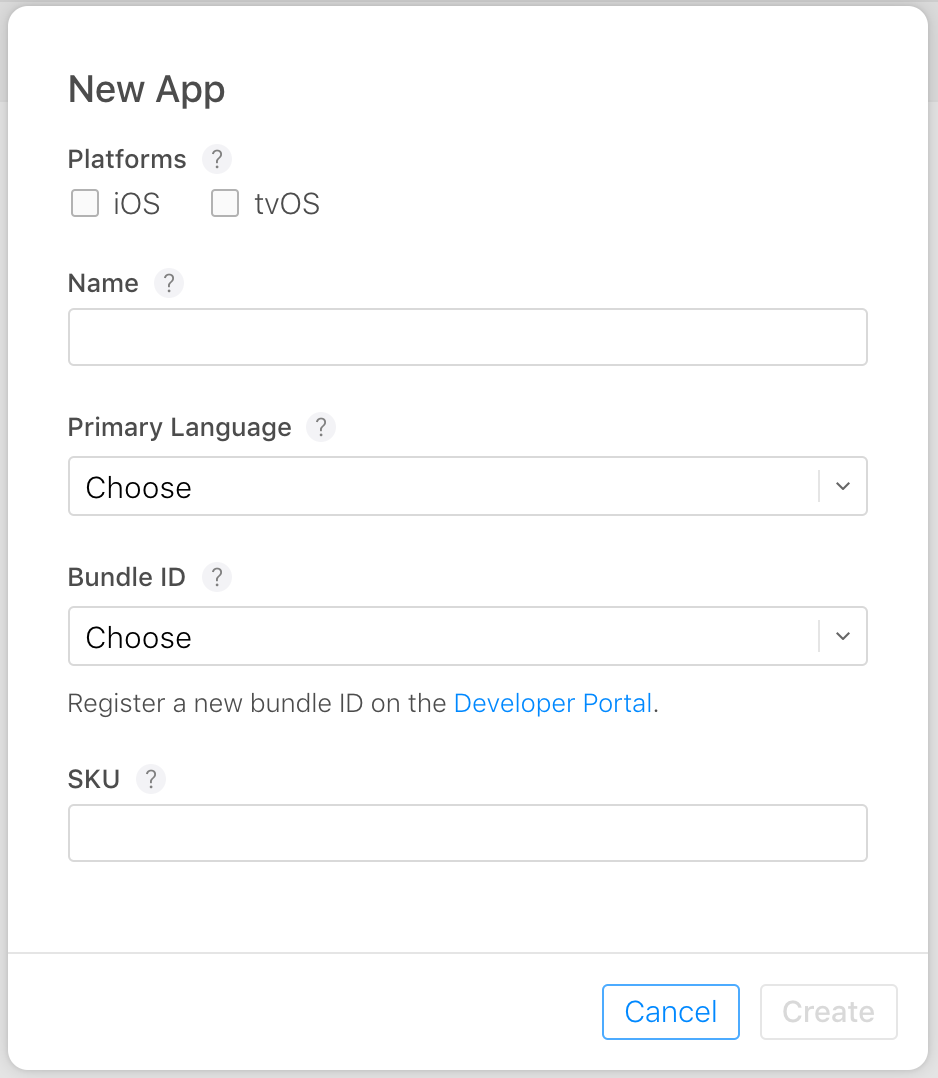
\includegraphics[scale=0.4]{iTunesConnectAppCreation}
\caption{Forma za kreiranje profila aplikacije na iTunes Connect web stranici}
\label{fig:iTunesConnectAppCreation}
\end{figure}

Isporuku programske potpore za App Store platformu implementiram pomoću fastlane dodatak \verb|deliver|\citep{fastlane:deliver}. Alat se inicijalizira pozivom \verb|fastlane deliver| \verb|init| naredbe. Naredba zahtijeva unos korisničkog imena i lozinke Apple Developer računa te unos identifikatora profila aplikacije. Identifikator je moguće dohvatiti korištenjem iTunes Connect stranice. Korištenjem stranice otvoriti profil aplikacije te locirati identifikator. Identifikator profila se nalazi pod poljem \verb|Apple ID|.

Naredba kreira nekoliko datoteka u \verb|fastlane| direktoriju. Tekstualna datoteka \verb|Deliverfile| pohranjuje podatke vezane uz objavu aplikacije na App Store platformi kao što su korisničko ime Apple Developer računa te identifikator aplikacije. Direktorij \verb|metadata| sadrži nekoliko dokumenata koji omogućavaju jednostavan unos podataka koji će se korisititi prilikom isporuke aplikacije na App Store platformu. Na primjer, pomoću dokumenta \verb|description.txt| je moguće specificirati opis aplikacije. Dodatno, moguće je kreirati zaseban opis za svaki jezik koji Apple podržava.

Sada je isporuku moguće obaviti jednostavno pozivom \verb|deliver| alata. Naravno, kreirana arhiva mora biti potpisana certifikatima i profilima za distribuciju na App Store platformi. Zbog navedenog kreiram novu shemu pomoću koje specificiram korištenje ispravnih certifikata i profila.

Staza u nastavku implementira objavu aplikacije na App Store platformu.

\begin{verbatim}
lane :release do
    match(type: "appstore")
    gym(scheme: “Production”)
    deliver
end
\end{verbatim}

Staza prvo dohvaća potrebne certifikate i profile, izgrađuje arhivu aplikacije te na kraju arhivu objavljuje koristeći deliver dodatak.

Nakon isporuke aplikacije je moguće pokrenuti proces objave. Prije objave, aplikacija mora proći Appleov pregled koji može trajati i do nekoliko tjedana. Zbog navedenog je preporučeno prije pokretanja procesa detaljno provjeriti ispravnost aplikacije te pročitati službene smjernice. Ako aplikacija prođe provjeru, onda ju je moguće objaviti korištenjem iTunes Connect web stranice.


\chapter{Usporedba alata za implementaciju kontinuirane integracije} \label{UsporedbaCIAlata_DodatakC}

\end{appendices}

\end{document}
